\documentclass{article}
\usepackage[utf8]{inputenc}
\usepackage{Preambles/preamble}

%~~~~~~~~~~~~~~~~~~~~~~~~~~~~~~~~~~~~~~~~~~~~~~~~~~~~~~~~~~~~~~~~~~~~~~~~~~~~~~~~~~~~~~~~~~~~~~%
%%%%%%%%%%%%%%%%%%%%%%%%%%%%%%%%%%%%%%%%%%%%%%%%%%%%%%%%%%%%%%%%%%%%%%%%%%%%%%%%%%%%%%%%%%%%%%%%
%                                                                                              % 
%             Template produced by Fergus Babb of the University of Nottingham, 2024           %
%                                                                                              %  
%%%%%%%%%%%%%%%%%%%%%%%%%%%%%%%%%%%%%%%%%%%%%%%%%%%%%%%%%%%%%%%%%%%%%%%%%%%%%%%%%%%%%%%%%%%%%%%%
%~~~~~~~~~~~~~~~~~~~~~~~~~~~~~~~~~~~~~~~~~~~~~~~~~~~~~~~~~~~~~~~~~~~~~~~~~~~~~~~~~~~~~~~~~~~~~~%

\begin{document}

%%%%%%%%%%%%%%%%%%%%%%%%%%%%%%%%%%%%%%%%%%%%%%%%%%%%%%%%%%%%%%%%%%%%%%%%%%%%%%%%%%%%%%%%%%%%%%%%
\title{Dynamic Parallel Maintaince of Strongly Connected Components in MPI}
%This isn't supposed to be for level of authorship, alphabetical is fine
\firstauthor{Soham Tripathy}
\firstID{CS20B073}
\firstemail{cs20b073@smail.iitm.ac.in}
\secondauthor{Name 2}
\secondID{Number ID 2}
\secondemail{ppyzzz@nottingham.ac.uk}
\supervisor{Professor. Rupesh Nasre}
\submitdate{\today}
\maketitle

\addtocounter{page}{-1}
\pagenumbering{roman}
\thispagestyle{empty}
%%%%%%%%%%%%%%%%%%%%%%%%%%%%%%%%%%%%%%%%%%%%%%%%%%%%%%%%%%%%%%%%%%%%%%%%%%%%%%%%%%%%%%%%%%%%%%%%

\newpage
\null\vspace{2in}
\begin{abstract}
This report explores the criticality of maintaining strongly connected components (SCCs) amidst dynamic changes in graph structures,
 emphasizing the efficiency of preserving SCCs during edge deletions and additions. Understanding the significance of SCCs in various applications,
 it becomes very challenging to recompute SCCs in response to changes in the graph structure. This requires efficient algorithms and optimization techniques
 to minimize the computational overhead and ensure real-time updates.
 Building upon prior research, we worked on extending an optimal algorithm tailored for this purpose. 
 Each facet of the algorithm deals with various cases of graph updates, which is elucidated with illustrative examples and accompanying pseudo code.
 
\vspace {1em}

Leveraging MPI for distributed parallel computation, we implement our algorithm,
 addressing encountered challenges and intricacies of the implementation process to facilitate comprehension of the code. 
 Detailed explanations of the design implementation, including the SCC tree construction, decremental and incremental maintenance, are provided.
 Rigorous testing on standard and specialized graphs, augmented with dynamic updates, is conducted, juxtaposing the performance against static SCC algorithms. 
 Results that are depicted through graphs and tables, are analyzed in the conclusion, offering insights and proposing avenues for future enhancements.
Additionally, the appendix elucidates the functionality and testing procedures of the implemented library, ensuring comprehensive understanding and usability.
\end{abstract}
\vspace{\fill}
\thispagestyle{empty}

%~~~~~~~~~~~~~~~~~~~~~~~~~~~~~~~~~~~~~~~~~~~~~~~~~~~~~~~~~~~~~~~~~~~~~~~~~~~~~~~~~~~~~~~~~~~~~~~

\newpage
\doublespacing
\tableofcontents
\singlespacing

%~~~~~~~~~~~~~~~~~~~~~~~~~~~~~~~~~~~~~~~~~~~~~~~~~~~~~~~~~~~~~~~~~~~~~~~~~~~~~~~~~~~~~~~~~~~~~~~
%Sections before Main Content of report

\newpage

\section*{Acronyms}\label{Acronyms}
\addcontentsline{toc}{subsection}{\textit{Acronyms}}
\begin{description}[style=unboxed,font=\small]
    \item[MPI:]\label{mpi} Message Passing Interface
    \item[SCC:]\label{scc} Strongly Connected Components
    \item[STN:]\label{stn} SCC-Tree Node
  \end{description}
\vspace{2em}

\listoffigures
\addcontentsline{toc}{subsection}{\textit{List of Figures}}
\vspace{2em}

\listoftables
\addcontentsline{toc}{subsection}{\textit{List of Tables}}
\vspace{2em}
\newpage
\null\vspace{2in}
\section*{Acknowledgements}\label{Acknowledgements}
\addcontentsline{toc}{subsection}{\textit{Acknowledgements}}
\vspace{2em}
I would like to express my heartfelt gratitude to \emph{Professor Rupesh Nasre}, Department of Computer Science and Engineering, Indian Institute of Technology, Madras for his invaluable guidance,
 unwavering support, and insightful feedback throughout the duration of this project. 
 His expertise and mentorship have been instrumental in shaping the direction of this work.

\vspace {1em}

 Additionally, I extend my sincere appreciation to the M.Tech students, \emph{Barenya Kumar Nandy} and \emph{Anurag Sao}, whose valuable insights, 
 references, and constant assistance have greatly enriched this endeavor.

\vspace {1em}

I would also like to thank the Indian Institute of Technology, Madras, for providing the necessary resources and infrastructure for the successful completion of this project.

\vspace{2em}

\hfill Soham Tripathy
\vspace{\fill}

%~~~~~~~~~~~~~~~~~~~~~~~~~~~~~~~~~~~~~~~~~~~~~~~~~~~~~~~~~~~~~~~~~~~~~~~~~~~~~~~~~~~~~~~~~~~~~~~
%Main Content sections start

\newpage
\pagenumbering{arabic}
\section*{Main Content}%So pdf viewers dont have everything as a subsection of preamble
\addcontentsline{toc}{part}{Main Content}


\section{Introduction} \label{Sec: Introduction}

Strongly connected components (SCCs) play a crucial role in graph theory, offering profound insights into the structure and connectivity of directed graphs. They are essential for understanding various real-world phenomena, ranging from social networks to computer algorithms.
\begin{itemize} 

    \item \textbf{Social Networks}:  In social networks like Facebook or Twitter, individuals form groups based on common interests, affiliations, or interactions. SCCs can help identify these tightly-knit communities within the network. For example, in a political analysis, identifying SCCs can reveal clusters of like-minded individuals or factions within a larger social network.
    \item \textbf{Transportation Networks}:  In transportation networks, such as road or railway systems, SCCs can represent regions where travel between any pair of locations is possible without leaving the component. This is crucial for optimizing routes, identifying traffic bottlenecks, and designing efficient public transportation systems.
    \item \textbf{Internet and Web Graphs:} The internet can be represented as a directed graph, where web pages are nodes and hyperlinks are edges. Identifying SCCs in this graph can reveal clusters of interconnected websites that share similar content or themes. This information is valuable for search engines to improve the relevance of search results and for analyzing the structure of the web.
    \item \textbf{Compiler Design}:  In compiler construction, analyzing the control flow graph of a program involves finding SCCs. This helps in optimizing code, identifying loops, and performing various program analyses, such as data-flow analysis and reaching definitions analysis.
    \item \textbf{Database Management}: In database systems, transactions between different parts of a database can be represented as a graph, where transactions are nodes and dependencies between them are edges. Detecting SCCs in these graphs helps in identifying sets of transactions that must be executed together or can be executed concurrently, improving database performance and transaction management.
\end{itemize}

In each of these cases, identifying strongly connected components provides valuable insights into the underlying structure and connectivity of the system, facilitating optimization, analysis, and decision-making processes.
Thus, developing efficient algorithms to find SCCs in directed graphs is a fundamental problem in graph theory and computer science.

There are various static linear time alogithms to find SCCs in a directed graph, such as Kosaraju's algorithm \cite{Kosaraju}, Tarjan's algorithm \cite{DBLP:journals/corr/abs-2201-07197}, that are partical and efficient for large-scale applications. However, these algorithms are designed for static graphs, where the graph structure does not change over time.
The problem of finding SCCs in a dynamic graph, where edges can be inserted or deleted, is more challenging and has received significant attention in recent years. The static algorithms are re-run on the entire graph to find the SCCs after each set of updates, which is computationally expensive and inefficient for large-scale graphs.

The goal of this project is to understand, formulate, and implement a dynamic parallel algorithm to find and maintain SCCs in a directed graph, where edges can be inserted or deleted dynamically. We aim to develop an efficient parallel algorithm that can handle large-scale graphs and leverage the computational power of modern multi-core processors and parallel computing platforms.

\section{Literature Review} \label{Sec: Literature Review}
\blindtext
\section{Theoretical Methodology}\label{Sec: Theoretical Methodology}
In this part, we elaborate on and enhance the algorithm proposed in \cite{scc_tree_reference}
for maintaining strongly connected components (SCCs) under a sequence of updates. 
The algorithm is designed to accommodate n vertices and m edges as input, proficiently manages the following operations:
\begin{itemize}
 \item  \textsc{Query}(u, v): Verifies whether both u and v belong to the same SCC.
 \item  \textsc{Delete}(u, v): Removes the edge from u to v.
\item  \textsc{Add}(u, v): Introduces the edge from u to v.
\end{itemize}

This algorithm achieves its objectives through the creation and continuous maintenance of a specialized data structure known as the SCC Tree, 
which is further explained in the subsequent section. 
Additionally, it employs an SCC mapping array to facilitate queries in constant time \textit{O(1)}.

The algorithm initiates with an initialization stage, wherein it constructs the proposed SCC tree 
and populates the SCC mapping array based on the identified strongly connected components within the graph. 
Subsequently, the process of constructing and maintaining these pivotal data structures under the delete and add updates is elaborated in the following sections, accompanied by their respective pseudo codes.

\subsection{Data Structures}\label{Subsec: Data Structures Theoretical}

In this section, we delve into a comprehensive exploration of the specialized data structures crucial to the functionality 
and efficiency of the algorithm. Through this detailed examination, we aim to provide clarity 
and insight into the design principles, operational mechanisms, and computational complexities of these structures.

\subsubsection{SCC Tree}\label{Subsubsec: SCC Tree}
The \hyperref[scc]{SCC} tree serves as a vital component in maintaining the internal connectivity of vertices within the strongly connected components of graph G. 
For each SCC identified in the graph, a corresponding SCC tree is constructed.

The node in the SCC tree corresponding to the label $R$ encapsulates a tuple that can be represented as $\text{\textsc{STN}}(R) = \lf( V, E \rt)$, 
where $V$ represents set of vertices and $E$ represents set of edges connecting them. We can thus informally infer that \textsc{STN}(R) holds some graph-like structure $G$.
We will refer to the vertex set of the SCC tree node labeled $R$ as $\text{\textsc{STN}}(R).V$ and the edge set as $\text{\textsc{STN}}(R).E$.
This encapsulation enables the SCC tree to maintain the connectivity of the vertices that are a part of the SCC labeled $R$,
also facilitating efficient traversal and update operations.

Each vertex $v \in V$ in the \hyperref[stn]{STN} of $R$ is a label uniquely associated with an SCC tree. 
This tree is a subtree of the SCC tree represented by the label $R$.
The SCC tree for a graph containing one vertex $v$ has only a single \hyperref[stn]{STN} represented as $\text{\textsc{STN}}(v) = (\{v\}, \emptyset)$.

\begin{figure}[H]
    \centering
    \begin{subfigure}[b]{0.4\textwidth}
        \centering
        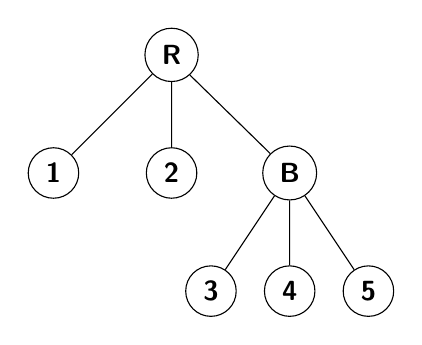
\begin{tikzpicture}[
            level distance=1.5cm,
            level 1/.style={sibling distance=1.5cm},
            level 2/.style={sibling distance=1cm},
            main node/.style={circle,draw,font=\sffamily\bfseries}]
                    % Define vertices
            \node[main node] (R) {R}
            child {node[main node] (1) {1}}
            child {node[main node] (2) {2}}
            child {node[main node] (B) {B}
                child {node[main node] (3) {3}}
                child {node[main node] (4) {4}}
                child {node[main node] (5) {5}}
            };
        \end{tikzpicture}
        \label{fig:example_scc_tree}
    \end{subfigure}
    \hfill
    \begin{subfigure}[b]{0.25\textwidth}
        \centering
        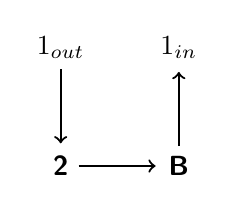
\begin{tikzpicture}[
            ->,shorten >=1pt,auto,node distance=1.5cm,
            thick,main node/.style={font=\sffamily\bfseries}]
            % Define vertices
        \node[main node] (1) {$1_{in}$};
        \node[main node] (11) [left of=1] {$1_{out}$};
        \node[main node] (2) [below of=11] {2};
        \node[main node] (B) [below of=1] {B};
        

        % Draw edges
        \path[every node/.style={font=\sffamily\small}]
            (11) edge (2)
            (2) edge (B)
            (B) edge (1);
        \end{tikzpicture}
        \caption{STN(R)}
        \label{fig:stn_r}
    \end{subfigure}
    \hfill 
    \begin{subfigure}[b]{0.25\textwidth}
        \centering
        \begin{tikzpicture}[
            ->,shorten >=1pt,auto,node distance=1.5cm,
            thick,main node/.style={font=\sffamily\bfseries}]
            % Define vertices
        \node[main node] (3) {$3_{in}$};
        \node[main node] (33) [left of=1] {$3_{out}$};
        \node[main node] (4) [below of=11] {4};
        \node[main node] (5) [below of=1] {5};
        

        % Draw edges
        \path[every node/.style={font=\sffamily\small}]
            (33) edge (4)
            (4) edge (5)
            (5) edge (3);
        \end{tikzpicture}
        \caption{STN(B)}
        \label{fig:stn_b}
    \end{subfigure}
    \caption{Example SCC Tree and its corresponding STNs}
    \label{fig:figure_with_subfigures}
\end{figure}

The SCC tree shown in \figureref{\ref{fig:figure_with_subfigures}}, can be represented by a collection of STNs as follows:
\begin{itemize}
    \item $\text{\textsc{STN}}(R)=(\{1,2,B\}, \{(1,2), (2,B), (B,1)\})$
    \item $\text{\textsc{STN}}(B)=(\{3,4,5\}, \{(3,4), (4,5), (5,3)\})$
    \item $\text{\textsc{STN}}(v)=\lf(\{v\}, \emptyset\rt) \forall v \in \{1,2,3,4,5\}$
\end{itemize}
The SCC tree represented by label $B$ contains the STNs of $\{B,3,4,5\}$, which form a subtree of the SCC tree represented by label $R$,
similarly, the SCC tree represented by labels $\{1,2\}$ also form $R$'s subtree.

\subsubsection{SCC Mapping Array}\label{Subsubsec: SCC Mapping Array}
In graph G, each vertex $v$ is inherently associated with a strongly connected component (SCC), denoted by its corresponding SCC label. 
The SCC mapping array effectively captures this relationship between vertices and their respective SCC labels.

Suppose vertex $v$ in graph $G$ belongs to the strongly connected component labeled as $R$.
 In that case, we express this association using the SCC mapping array notation as $\text{\textsc{SM}}_{G}(v)=R$. 
 This signifies that vertex $v$ is mapped to the SCC labeled as $R$ within the context of the graph $G$.


\subsection{Definitions}\label{Subsec: Definitions Theoretical}
In this section, we establish key definitions that form the foundation of the algorithms presented subsequently. 
These definitions are instrumental in understanding the intricacies of the algorithms and their associated data structures.

\subsubsection{\textsc{FindScc}(G)}\label{Subsubsec: FindScc}
For a given graph $G$, let $V(G)$ represent the set of vertices of graph $G$.
We consider $k$ set of vertices as $U_i \forall i \in [1,k]$ such that it satisfies that following conditions:
\begin{itemize}
    \item $\bigcup\limits_{i=1}^{i=k}U_i = V(G)$
    \item $U_i \cap U_j = \emptyset$  $\forall i, j \in [1,k] | i \neq j$
    \item For each $U_i$, we say $\forall v, u \in U_i | v \neq u$, $\text{\textsc{Query}}(u, v) = true$.
    \item For any $U_i$ and $U_j$ such that $i \neq j$, $\forall v \in U_i$ and $\forall u \in U_j$, $\text{\textsc{Query}}(u, v) = false$.
\end{itemize}
We define the function \textsc{FindScc}(G) as the process of identifying the set of vertices $U_i$ that satisfies the above conditions.
The function \textsc{FindScc}(G) is instrumental in identifying the strongly connected components within the graph $G$.
We can do this by using any standard linear time algorithm, some of which are mentioned in \cite{find_scc_algorithm}, \cite{Kosaraju}, and \cite{DBLP:journals/corr/abs-2201-07197}.

\subsubsection{\textsc{Condense}(G)}\label{Subsubsec: Condense}

We define \textsc{Condense}(G) as condensing the graph $G$ into a new graph $G'$, where each vertex in $G'$ represents a strongly connected component in $G$,
$ie.$ $V(G') = \{\text{\textsc{SM}}_G(v) | v \in V(G)\}$.
The edges in $G'$ are such that if there is an edge from $u$ to $v$ in $G$, and $u$ and $v$ belong to different strongly connected components in $G$,
then there is an edge from the strongly connected component containing $u$ to the strongly connected component containing $v$ in $G'$. 
Therefore, a edge $(u, v) \in E(G) | \text{\textsc{Query}}(u, v) = false$ correponds to an edge $(\text{\textsc{SM}}_{G}(u), \text{\textsc{SM}}_{G}(v)) \in E(G')$.

\begin{algorithm}[H]
    \SetAlgoLined
    \KwData{G}
    \KwResult{G'}
    U = \text{\textsc{FindScc}}(G)\;
    \For {$U_i \in U$} {
        L = new label\;
        \For {$v \in U_i$} {
            $\text{\textsc{SM}}_G(v)$ = L\;
        }
        $V(G') = V(G')\cup L$
    }
    \For {$(u, v) \in E(G)$} {
        \If {$\text{\textsc{Query}}(u, v) = false$} {
            $E(G') = E(G') \cup (\text{\textsc{SM}}_G(u), \text{\textsc{SM}}_G(v))$
        }
    }
    \caption{\textsc{Condense}(G)}
\end{algorithm}

\subsubsection{\textsc{Split}(G,d)}\label{Subsubsec: Split}
Consider any graph G with a set of vertices $V(G)$ and a set of edges $E(G)$ such that $|\text{\textsc{FindScc}}(G)| = 1$.
Let $\exists d \in V(G)$ that can be split into two vertices $d_{in}$ and $d_{out}$ producing a new graph $G'$ 
such that any edge incident on $d$ is now incident on $d_{in}$ and any edge originating from $d$ is now originating from $d_{out}$.

\begin{algorithm}[H]
    \SetAlgoLined
    \KwData{G, d}
    \KwResult{G'}
    $V(G') = (V(G) \setminus \{d\}) \cup \{d_{in}, d_{out}\}$\;
    \For {$(u, v) \in E(G)$} {
        \If {$v = d$} {
            $E(G') = E(G') \cup (u, d_{in})$
        }
        \textbf{else} \If {$u = d$} {
            $E(G') = E(G') \cup (d_{out}, v)$
        }
        \Else {
            $E(G') = E(G') \cup (u, v)$
        }
    }
    \caption{\textsc{Split}(G,d)}
\end{algorithm}

\subsubsection{\textsc{Merge}(G, s, t, d)}\label{Subsubsec: Merge}
Let there be a graph $G$ such that it has a source vertex $s$ and a sink vertex $t$.
We define \textsc{Merge}(G,s,t, d) as merging the vertices $s$ and $t$ into vertex $d$ in the graph $G$ to produce a new graph $G'$.
This operation is the inverse of the \textsc{Split}(G, d) operation.

\begin{algorithm}[H]
    \SetAlgoLined
    \KwData{G,s,t,d}
    \KwResult{G'}
    $V(G') = V(G) \setminus \{t, s\} \cup \{d\}$\;
    \For {$(u, v) \in E(G)$} {
        \If {$v = t$} {
            $E(G') = E(G') \cup (u, d)$
        }
        \textbf{else} \If {$u = s$} {
            $E(G') = E(G') \cup (d, v)$
        }
        \Else {
            $E(G') = E(G') \cup (u, v)$
        }
    }
    \caption{\textsc{Merge}(G,s,t,d)}
\end{algorithm}

\subsubsection{\textsc{Unreachable}(G,s,t)}\label{Subsubsec: Unreachable}

Let there be a graph $G$ such that it has a source vertex $s$ and a sink vertex $t$.
A vertex $v$ is said to reachable if there exists a path from $s$ to $v$ and a path from $v$ to $t$.
We define the function \textsc{Unreachable}(G,s,t) as the process of identifying the set of vertices that are unreachable in $G$.

\begin{algorithm}[H]
    \SetAlgoLined
    \KwData{G, s, t}
    \KwResult{U}
    $U = \emptyset$\;
    $G' =$ \textsc{Merge}(G, s, t, d)\;
    $S = \text{\textsc{FindScc}}(G')$\;
    $R = \emptyset$\;
    \For {$U_i \in S$} {
        \If {$s \in U_i$} {
            $R = U_i$
        }
    }
    $U = V(G) \setminus R$\;
    \caption{\textsc{Unreachable}(G,s,t)}
\end{algorithm}


% subsection of construction of scc tree
\subsection{Constructing SCC Tree}

We will look at the construction of the SCC tree for the graph shown in \figureref{\ref{fig:graph1}}.
We start by finding all the SCCs of the graph and then construct the SCC-Tree for each SCC in it.
In the process of finding all the SCCs, we would also fill the SCC mapping array. 
A special tree node \textsc{STN}(M), called the master node would preserve the connectivity of the SCCs (condesed form of the original graph).

\begin{algorithm}[H]
    \SetAlgoLined
    \KwData{G}
    \KwResult{SCC mapping, \textsc{SccTree}s, \textsc{STN}(M)}
    $SM_{G} = \emptyset, \textsc{SccTree} = \emptyset$\;
    $S = \textsc{FindSccs}(G)$\;
    $V_l = \emptyset, E_l = E(G)$\;
    \For {each $s \in S$} {
        $L_s = \textsc{Label}(s)$\;
        $G_s = G \cap s$\;
        $\textsc{SccTree}(L_s) = \textsc{MakeTree}(G_s, L_s)$\;
        \For {each $v \in s$} {
            $SM_{G}(v) = L_s$\;
        }
        $V_l = V \cup \{L_s\}$\;
        $E_l = E_l - \{e \in E(G_s)\}$\;
    }
    $\textsc{STN}(M) = (V_l, E_l)$\;
    \Return $SM_{G}, \textsc{SccTree}s, \textsc{STN}(M) = (V_l, E_l)$\;

    \caption{\textsc{ConstructDS}(G)}
\end{algorithm}

Suppose we have a strongly connected graph $G$, the SCC Tree for the graph is constructed as follows:
\begin{itemize}
    \item If $|V(G)| = 1$ and $v \in V(G)$, then the SCC tree is $SCC(v) = STN(v) = (\{v\}, \emptyset)$.
    \item If $|V(G)| > 1$ and $d \in V(G)$, then the root SCC tree node would contain the graph \textsc{Condense}(\textsc{Split}($G, d$)), 
    and for each SCC in the graph \textsc{Condense}(\textsc{Split}($G, d$)), we add its SCC-tree as a subtree of R, with 
    exception that we would add only one tree for vertex $d$ instead of $d_{in}$ and $d_{out}$.
\end{itemize}

%algorithm
\begin{algorithm}[H]
    \SetAlgoLined
    \KwData{G | G is strongly connected, L | label of the root node}
    \KwResult{\textsc{SccTree(L)}}
    $v = random(V(G))$\;
    $\textsc{SccTree}(L) = \emptyset$\;
    \If {$|V(G)| = 1$} {
        $\textsc{STN}(L) = (\{v\}, \emptyset)$\;
        $\textsc{SccTree}(L) = \textsc{STN}(L)$\;
        \Return \textsc{SccTree}(L)\;
    }
    $G' = \textsc{Split}(G, v)$\;
    $S = \textsc{FindSccs}(G')$\;
    \For {each $s \in S$ and $v_{in} \not \in s$} {
        $L_s = \textsc{Label}(s)$\;
        $G_s = G' \cap s$\;
        $\textsc{SccTree}(L_s) = \textsc{MakeTree}(G_s, L_s)$\;
        $\textsc{SccTree}(L) = \textsc{SccTree}(L) \cup \textsc{SccTree}(L_s)$\;
    }
    $\textsc{STN}(L) = \textsc{Condense}(G')$\;
    $\textsc{SccTree}(L) = \textsc{SccTree}(L) \cup \textsc{STN}(L)$\;
    \Return \textsc{SccTree}(L)\;

    \caption{\textsc{MakeTree(G, L)}}
\end{algorithm}

We can understand the algorithm by looking at the following figures.
In \figureref{\ref{fig:graph1_and_condensed_graph1}}, we have the graph $G$, which is strongly connected.
Its condensed form would contain a single node $R$. The SCC mapping array would map all the nodes to $R$ and the master node 
would contain the graph in \figureref{\ref{fig:condensed_graph1}}.
\begin{figure}[H]
    \centering
    \begin{subfigure}{0.45\textwidth}
        \centering
        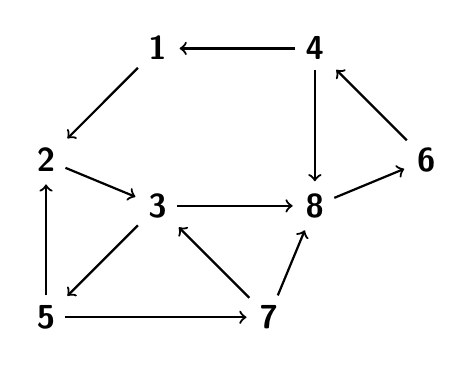
\begin{tikzpicture}[->,shorten >=1pt,auto,node distance=2cm,
            thick,main node/.style={font=\sffamily\large\bfseries}]

        % Define vertices
        \node[main node] (1) {1};
        \node[main node] (2) [below left of=1] {2};
        \node[main node] (3) [below of=1] {3};
        \node[main node] (4) [right of=1] {4};
        \node[main node] (5) [below left of=3] {5};
        \node[main node] (6) [below right of=4] {6};
        \node[main node] (7) [below right of=3] {7};
        \node[main node] (8) [right of=3] {8};
        

        % Draw edges
        \path[every node/.style={font=\sffamily\small}]
            (1) edge (2)
            (2) edge (3)
            (3) edge (5)
            (3) edge (8)
            (4) edge (1)
            (4) edge (8)
            (5) edge (2)
            (5) edge (7)
            (6) edge (4)
            (7) edge (3)
            (7) edge (8)
            (8) edge (6);

        \end{tikzpicture}
        \caption{Graph 1}
        \label{fig:graph1}
    \end{subfigure}
    \hfill
    \begin{subfigure}{0.45\textwidth}
        \centering
        
\begin{tikzpicture}[->,shorten >=1pt,auto,node distance=2cm,
            thick,main node/.style={circle,draw,font=\sffamily\bfseries}]

        % Define vertices
        \node[main node] (R) {R};

        \end{tikzpicture}
        \caption{condensed graph 1}
        \label{fig:condensed_graph1}
    \end{subfigure}
    \caption{Graph 1 and its condensed graph}
    \label{fig:graph1_and_condensed_graph1}
\end{figure}

After the strongly connected components of the graph are indentified, they are individually processed by the 
\textsc{MakeTree} algorithm. The algorithm starts by selecting a random vertex from the SCC and then splits the graph
on that vertex. The split graph is then condensed and the strongly connected components of the condensed graph are found. 
This is illustrated in \figureref{\ref{fig:scc_r_split_and_condensed_graph1}}, where we can see the condensed components $A$ and $B$.
The condesed graph in \figureref{\ref{fig:condensed_scc_r_split}} is stored in the \textsc{STN} of the root node $R$.
\begin{figure}[H]
    \centering
    \begin{subfigure}{0.45\textwidth}
        \centering
        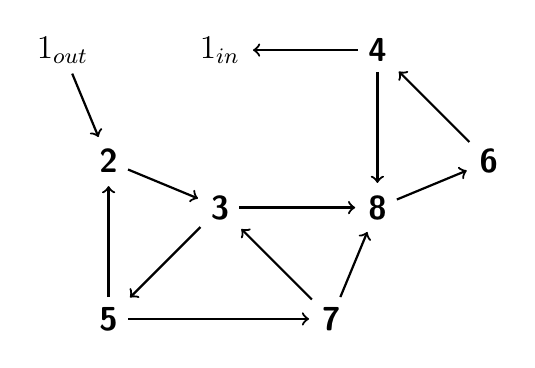
\begin{tikzpicture}[->,shorten >=1pt,auto,node distance=2cm,
            thick,main node/.style={font=\sffamily\large\bfseries}]

        % Define vertices
        \node[main node] (1) {$1_{in}$};
        \node[main node] (11) [left of=1] {$1_{out}$};
        \node[main node] (2) [below left of=1] {2};
        \node[main node] (3) [below of=1] {3};
        \node[main node] (4) [right of=1] {4};
        \node[main node] (5) [below left of=3] {5};
        \node[main node] (6) [below right of=4] {6};
        \node[main node] (7) [below right of=3] {7};
        \node[main node] (8) [right of=3] {8};
        

        % Draw edges
        \path[every node/.style={font=\sffamily\small}]
            (11) edge (2)
            (2) edge (3)
            (3) edge (5)
            (3) edge (8)
            (4) edge (1)
            (4) edge (8)
            (5) edge (2)
            (5) edge (7)
            (6) edge (4)
            (7) edge (3)
            (7) edge (8)
            (8) edge (6);

        \end{tikzpicture}
        \caption{SCC(R) split on 1}
        \label{fig:scc_r_split}
    \end{subfigure}
    \hfill
    \begin{subfigure}{0.45\textwidth}
        \centering
        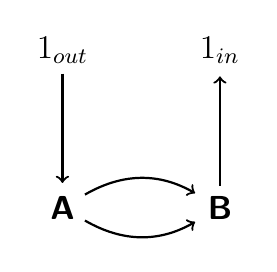
\begin{tikzpicture}[->,shorten >=1pt,auto,node distance=2cm,
            thick,main node/.style={font=\sffamily\large\bfseries}]

        % Define vertices
        \node[main node] (1) {$1_{in}$};
        \node[main node] (11) [left of=1] {$1_{out}$};
        \node[main node] (A) [below of=11] {A};
        \node[main node] (B) [below of=1] {B};
        

        % Draw edges
        \path[every node/.style={font=\sffamily\small}]
            (11) edge (A)
            (A) edge[bend left] (B)
            (A) edge[bend right] (B)
            (B) edge (1);

        \end{tikzpicture}
        \caption{condensed graph}
        \label{fig:condensed_scc_r_split}
    \end{subfigure}
    \caption{SCC(R) split on 1 and its condensed graph}
    \label{fig:scc_r_split_and_condensed_graph1}
\end{figure}

The \textsc{MakeTree} algorithm then processes all the condensed components of the split graph in a recursive manner.
The condensed component $A$ is split on 2, as in \figureref{\ref{fig:scc_a_split_and_condensed_graph1}}, and the 
condensed component $B$ is split on 4, as shown in \figureref{\ref{fig:scc_b_split_and_condensed_graph1}}. The 
component $A$ contains $C$ which is split on 3, as shown in \figureref{\ref{fig:scc_c_split_and_condensed_graph1}}.
The condesed graphs in \figureref{\ref{fig:condensed_scc_a_split}}, \figureref{\ref{fig:condensed_scc_b_split}}, and
\figureref{\ref{fig:condensed_scc_c_split}} are stored in the \textsc{STN} of $A$, $B$, and $C$ respectively.
\begin{figure}[H]
    \centering
    \begin{subfigure}{0.45\textwidth}
        \centering
        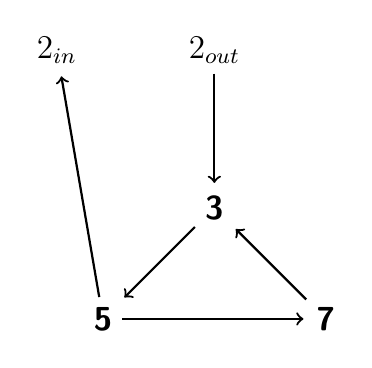
\begin{tikzpicture}[->,shorten >=1pt,auto,node distance=2cm,
            thick,main node/.style={font=\sffamily\large\bfseries}]

        % Define vertices
        \node[main node] (2) {$2_{out}$};
        \node[main node] (22) [left of=2] {$2_{in}$};
        \node[main node] (3) [below of=2] {3};
        \node[main node] (5) [below left of=3] {5};
        \node[main node] (7) [below right of=3] {7};
        

        % Draw edges
        \path[every node/.style={font=\sffamily\small}]
            (2) edge (3)
            (3) edge (5)
            (5) edge (22)
            (5) edge (7)
            (7) edge (3);

        \end{tikzpicture}
        \caption{SCC(A) split on 2}
        \label{fig:scc_a_split}
    \end{subfigure}
    \hfill
    \begin{subfigure}{0.45\textwidth}
        \centering
        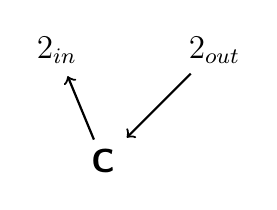
\begin{tikzpicture}[->,shorten >=1pt,auto,node distance=2cm,
            thick,main node/.style={font=\sffamily\large\bfseries}]

        % Define vertices
        \node[main node] (2) {$2_{out}$};
        \node[main node] (22) [left of=2] {$2_{in}$};
        \node[main node] (C) [below left of=2] {C};
        

        % Draw edges
        \path[every node/.style={font=\sffamily\small}]
            (2) edge (C)
            (C) edge (22);

        \end{tikzpicture}
        \caption{condensed graph}
        \label{fig:condensed_scc_a_split}
    \end{subfigure}
    \caption{SCC(A) split on 2 and its condensed graph}
    \label{fig:scc_a_split_and_condensed_graph1}
\end{figure}

\begin{figure}[H]
    \centering
    \begin{subfigure}{0.45\textwidth}
        \centering
        \begin{tikzpicture}[->,shorten >=1pt,auto,node distance=2cm,
            thick,main node/.style={font=\sffamily\large\bfseries}]

        % Define vertices
        \node[main node] (4) {$4_{in}$};
        \node[main node] (44) [left of=1] {$4_{out}$};
        \node[main node] (6) [below of=1] {6};
        \node[main node] (8) [below of=11] {8};
        

        % Draw edges
        \path[every node/.style={font=\sffamily\small}]
            (44) edge (8)
            (8) edge (6)
            (6) edge (4);

        \end{tikzpicture}
        \caption{SCC(B) split on 4}
        \label{fig:scc_b_split}
    \end{subfigure}
    \hfill
    \begin{subfigure}{0.45\textwidth}
        \centering
        \begin{tikzpicture}[->,shorten >=1pt,auto,node distance=2cm,
            thick,main node/.style={font=\sffamily\large\bfseries}]

        % Define vertices
        \node[main node] (4) {$4_{in}$};
        \node[main node] (44) [left of=1] {$4_{out}$};
        \node[main node] (6) [below of=1] {6};
        \node[main node] (8) [below of=11] {8};
        

        % Draw edges
        \path[every node/.style={font=\sffamily\small}]
            (44) edge (8)
            (8) edge (6)
            (6) edge (4);

        \end{tikzpicture}
        \caption{condensed graph}
        \label{fig:condensed_scc_b_split}
    \end{subfigure}
    \caption{SCC(B) split on 4 and its condensed graph}
    \label{fig:scc_b_split_and_condensed_graph1}
\end{figure}

\begin{figure}[H]
    \centering
    \begin{subfigure}{0.45\textwidth}
        \centering
        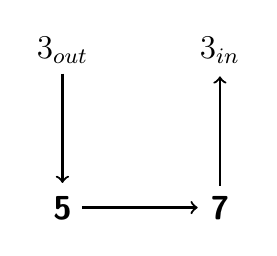
\begin{tikzpicture}[->,shorten >=1pt,auto,node distance=2cm,
            thick,main node/.style={font=\sffamily\large\bfseries}]

        % Define vertices
        \node[main node] (3) {$3_{in}$};
        \node[main node] (33) [left of=3] {$3_{out}$};
        \node[main node] (5) [below of=33] {5};
        \node[main node] (7) [below of=3] {7};
        

        % Draw edges
        \path[every node/.style={font=\sffamily\small}]
            (33) edge (5)
            (5) edge (7)
            (7) edge (3);

        \end{tikzpicture}
        \caption{SCC(C) split on 3}
        \label{fig:scc_c_split}
    \end{subfigure}
    \hfill
    \begin{subfigure}{0.45\textwidth}
        \centering
        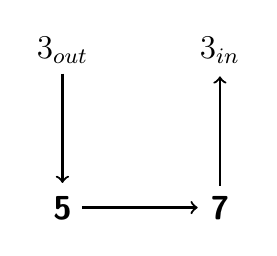
\begin{tikzpicture}[->,shorten >=1pt,auto,node distance=2cm,
            thick,main node/.style={font=\sffamily\large\bfseries}]

        % Define vertices
        \node[main node] (3) {$3_{in}$};
        \node[main node] (33) [left of=3] {$3_{out}$};
        \node[main node] (5) [below of=33] {5};
        \node[main node] (7) [below of=3] {7};
        

        % Draw edges
        \path[every node/.style={font=\sffamily\small}]
            (33) edge (5)
            (5) edge (7)
            (7) edge (3);

        \end{tikzpicture}
        \caption{condensed graph}
        \label{fig:condensed_scc_c_split}
    \end{subfigure}
    \caption{SCC(C) split on 3 and its condensed graph}
    \label{fig:scc_c_split_and_condensed_graph1}
\end{figure}

The figure \figureref{\ref{fig:scc_tree_graph1}} shows the SCC tree for the graph in \figureref{\ref{fig:graph1}}.
The SCC tree is constructed by the \textsc{MakeTree} algorithm, which recursively processes the condensed components of the split graph.
The child of each parent node in the SCC tree is a node present in the \textsc{STN} of the parent node.
\\$\textsc{SccTree(R)} = \textsc{STN}\text{'s of } \{R, 1, A, 2, C, 3, 5, 7, B, 4, 6, 8\}$


\begin{figure}[H]
    \centering
    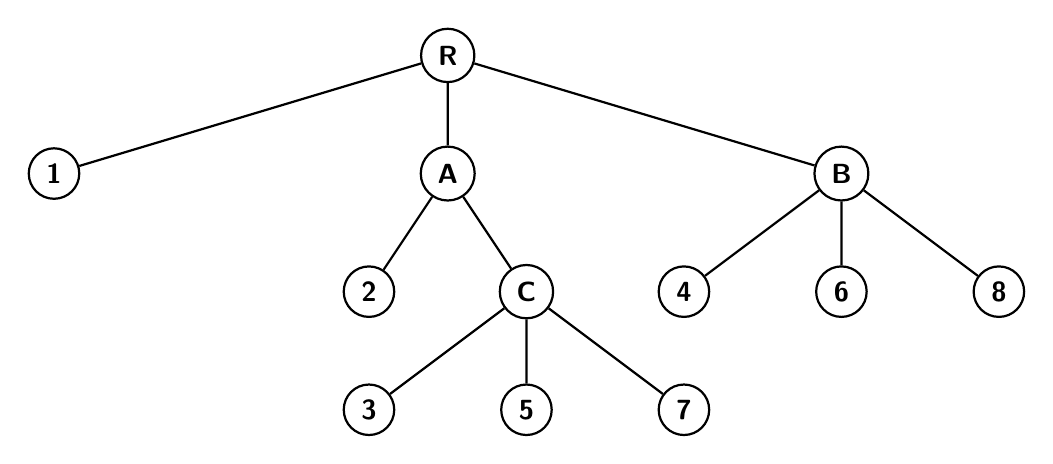
\begin{tikzpicture}[level distance=1.5cm,
                        level 1/.style={sibling distance=5cm},
                        level 2/.style={sibling distance=2cm},
                        thick,main node/.style={circle,draw,font=\sffamily\bfseries}]

      % Define vertices
      \node[main node] (R) {R}
        child {node[main node] (1) {1}}
        child {node[main node] (A) {A}
          child {node[main node] (2) {2}}
          child {node[main node] (C) {C}
            child {node[main node] (3) {3}}
            child {node[main node] (5) {5}}
            child {node[main node] (7) {7}}
          }
        }
        child {node[main node] (B) {B}
          child {node[main node] (4) {4}}
          child {node[main node] (6) {6}}
          child {node[main node] (8) {8}}
        };

    \end{tikzpicture}
    \caption{SCC Tree of Graph \ref{fig:graph1}}
    \label{fig:scc_tree_graph1}
\end{figure}



\subsection{Decremental Maintaince of SCC Tree}\label{Subsec: Decremental Maintaince of SCC Tree}

In this section, we delve into the decremental maintenance of the SCC tree under the delete operation.
As mentioned earlier, the \textsc{Delete}(u, v) operation removes the edge from vertex $u$ to vertex $v$ in the graph $G$.
This deletion operation necessitates the corresponding update in the SCC tree to maintain the internal connectivity of the vertices within the strongly connected components.
The deletion may also introduce new strongly connected components that may be formed due to the decomposition of the earlier SCCs.

Given, a graph $G$ and an edge $(u, v)$ is to be deleted from the graph $G$. Suppose if the vertex $u$ and $v$ belong to different strongly connected component, 
then the deletion of the edge $(u, v)$ will not affect any SCC tree. It would also not introduce any new SCCs, since the edge $(u, v)$ was not a part of any SCC.
In this case, we can simply remove the edge $(u, v)$ from the edge set of the master node.

However, if the vertices $u$ and $v$ belong to the same strongly connected component, then the deletion of the edge $(u, v)$ may introduce new SCCs or change the internal connectivity of the SCC tree.
Therefore, while we delete an edge $(u, v)$, we first must identify the SCC tree node that contains the edge $(u, v)$. This can be done by 
finding the lowest commen ancestor of the vertices $u$ and $v$ in the SCC tree. We then proceed to delete the edge from the identified node.

\begin{algorithm}[H]
    \SetAlgoLined
    \KwData{G, u, v}
    \KwResult{G'}
    \If {$\text{\textsc{Query}}(u, v) = false$} {
        $\text{\textsc{STN}}(M).E = \text{\textsc{STN}}(M).E \setminus \{(u, v)\}$\;
        \textbf{return}\;
    }
    $L = \text{\textsc{LCA}}(u, v)$\;
    $\text{\textsc{STN}}(L).E = \text{\textsc{STN}}(L).E \setminus \{(u, v)\}$\;
    \textsc{UpdateSCCTree}(L)\;
    \caption{\textsc{Delete}(G, u, v)}
\end{algorithm}

After the deletion of the edge $(u, v)$, we must ensure that the SCC tree is updated to reflect the changes in the internal connectivity of the vertices.
The updates ensures that the every vertex in each SCC tree node is reachable from the vertex $d_{out}$ and $d_{in}$, where $d$ is the vertex that was split to construct the SCC tree node,
we refer \secref{\ref{Subsubsec: Unreachable}} for the definition.

The following steps are performed to update the SCC tree after the deletion of the edge $(u, v)$ which belongs to the SCC tree node $L$, and $d$ is the vertex that was split to construct the SCC tree node $L$:
\begin{itemize}
    \item The unreachable vertices are removed form the SCC tree node $L$, and are added in the vertex set of the SCC tree node $p(L)$, where $p(L)$ denotes parent node of $L$.
If $L$ is the root node, then the unreachable vertices form new SCC-tree's, and thus updating the master node and the SCC mapping array.
    \item If vertices were removed from the SCC tree node $L$, then repeat the above steps for the parent node of $L$. This process stops when $L$ is the root node of the SCC tree, we then update the master node and the SCC mapping array.
    \item If unreachable vertices are present, then we expose the connectivity of these vertices to the parent node of $L$. This can be achieved by transferring
the edges that were a part of the unreachable vertices in $L$ to the parent node and also updating the edges in the edge set of the parent node that involved the unreachable vertices, which were a part of $L$.
This can be seen in \figureref{\ref{fig:tree_node_r_graph_exposed1}}, further details can be found in \secref{\ref{Subsubsec: Deleting Edge from the Root Node}} and \secref{\ref{Subsubsec: Deleting Edge from an Internal Node}}.
\end{itemize}

\begin{algorithm}[H]
    \SetAlgoLined
    \KwData{L | SCC Tree Node}
    \KwResult{Updated SCC Tree}
    $U = \text{\textsc{Unreachable}}(L, d_{in}, d_{out})$\;
    \textbf{if} {$U == \emptyset$} \textbf{then} \textbf{return}\;
    $E\_to\_expose = \emptyset$\;
    \hspace{1em}\\    \{Step 1: Removing vertices and edges\} \\
    \For {$v \in U$} {
        $\text{\textsc{STN}}(L).V = \text{\textsc{STN}}(L).V \setminus \{v\}$\;
    }
    \For {$(u, v) \in \text{\textsc{STN}}(L).E$} {
        \If {$u \in U$ or $v \in U$} {
            $\text{\textsc{STN}}(L).E = \text{\textsc{STN}}(L).E \setminus \{(u, v)\}$\;
            $E\_to\_expose = E\_to\_expose \cup \{(u, v)\}$\;
        }
    }
    \phantom{text}\\   \{Step 2: Exposing the connectivity\} \\
    \If {$L == \text{Root}$} {
        $p(L) = \textsc{STN}(M)$\;
    }
    \For {$(u, v) \in \textsc{STN}(p(L)).E$} {
        \For {$k \in U$} {
            $P = \textsc{SccTree}(k).Label$\;
            \If {$u \in P$} {
                $\textsc{STN}(p(L)).E = \textsc{STN}(p(L)).E \setminus \{(u, v)\}$\;
                $\textsc{STN}(p(L)).E = \textsc{STN}(p(L)).E \cup \{(k, v)\}$\;
            }
            \If {$v \in P$} {
                $\textsc{STN}(p(L)).E = \textsc{STN}(p(L)).E \setminus \{(u, v)\}$\;
                $\textsc{STN}(p(L)).E = \textsc{STN}(p(L)).E \cup \{(u, k)\}$\;
            }
        }
    }
    $\textsc{STN}(p(L)).E = \textsc{STN}(p(L)).E \cup E\_to\_expose$\;
    $\textsc{STN}(p(L)).V = \textsc{STN}(p(L)).V \cup U$\;
    \phantom{text}\\   \{ Step 3: Recursion (or) Updating the SCC Mapping Array\} \\
    \If {$L \neq \text{Root}$} {
        \textsc{UpdateSCCTree}(p(L))\;
    }
    \Else {
        \For {$v \in U$} {
            \For {$u \in \textsc{SccTree}(v).Label$} {
                \If {$\textsc{STN}(u).E == \emptyset$} {
                    $\textsc{SM}_G(u) = v$\;
                }
            }
        }
    }

    \caption{\textsc{UpdateSCCTree}(L)}
\end{algorithm}


\subsubsection{Deleting Edge from the Root Node}\label{Subsubsec: Deleting Edge from the Root Node}

\begin{figure}[H]
    \centering
    \begin{subfigure}{0.45\textwidth}
        \centering
        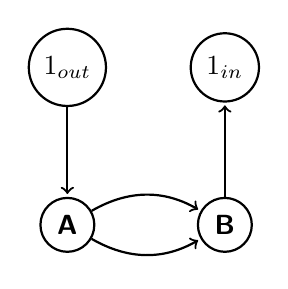
\begin{tikzpicture}[->,shorten >=1pt,auto,node distance=2cm,
            thick,main node/.style={circle,draw,font=\sffamily\bfseries}]

        % Define vertices
        \node[main node] (1) {$1_{in}$};
        \node[main node] (11) [left of=1] {$1_{out}$};
        \node[main node] (A) [below of=11] {A};
        \node[main node] (B) [below of=1] {B};
        

        % Draw edges
        \path[every node/.style={font=\sffamily\small}]
            (11) edge (A)
            (A) edge[bend left] (B)
            (A) edge[bend right] (B)
            (B) edge (1);

        \end{tikzpicture}
        \caption{Graph in SCC Tree Node R}
        \label{fig:tree_node_r_graph}
    \end{subfigure}
    \hfill
    \begin{subfigure}{0.45\textwidth}
        \centering
        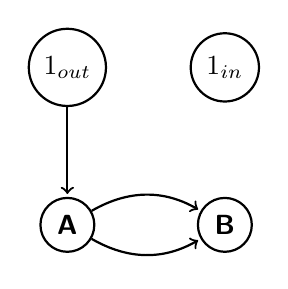
\begin{tikzpicture}[->,shorten >=1pt,auto,node distance=2cm,
            thick,main node/.style={circle,draw,font=\sffamily\bfseries}]

        % Define vertices
        \node[main node] (1) {$1_{in}$};
        \node[main node] (11) [left of=1] {$1_{out}$};
        \node[main node] (A) [below of=11] {A};
        \node[main node] (B) [below of=1] {B};
        

        % Draw edges
        \path[every node/.style={font=\sffamily\small}]
            (11) edge (A)
            (A) edge[bend left] (B)
            (A) edge[bend right] (B);

        \end{tikzpicture}
        \caption{Graph after deleting edge 4 to 1}
        \label{fig:graph_after_dedge_4_to_1}
    \end{subfigure}
    \caption{Graph in SCC Tree Node R after deleting edge 4 to 1}
    \label{fig:tree_node_r_graph_after_dedge1}
\end{figure}


\begin{figure}[H]
    \centering
    \begin{subfigure}{0.45\textwidth}
        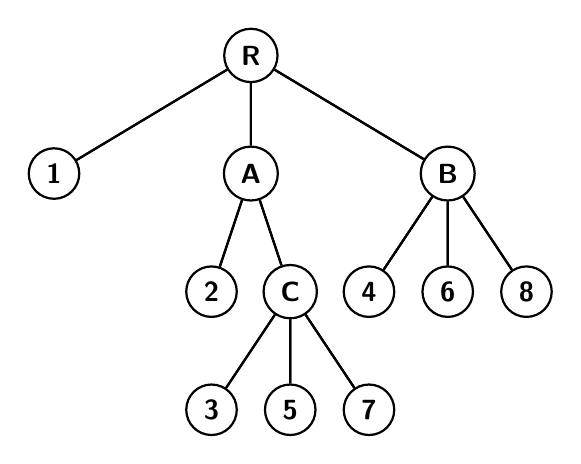
\begin{tikzpicture}[level distance=1.5cm,
                            level 1/.style={sibling distance=2.5cm},
                            level 2/.style={sibling distance=1cm},
                            thick,main node/.style={circle,draw,font=\sffamily\bfseries}]

        % Define vertices
        \node[main node] (R) {R}
            child {node[main node] (1) {1}}
            child {node[main node] (A) {A}
            child {node[main node] (2) {2}}
            child {node[main node] (C) {C}
                child {node[main node] (3) {3}}
                child {node[main node] (5) {5}}
                child {node[main node] (7) {7}}
            }
            }
            child {node[main node] (B) {B}
            child {node[main node] (4) {4}}
            child {node[main node] (6) {6}}
            child {node[main node] (8) {8}}
            };

        % Draw edges
        \path[every node/.style={font=\sffamily\small}]
            (R) edge (1)
            (R) edge (A)
            (R) edge (B)
            (A) edge (2)
            (A) edge (C)
            (B) edge (4)
            (B) edge (6)
            (B) edge (8)
            (C) edge (3)
            (C) edge (5)
            (C) edge (7);

        \end{tikzpicture}
        \caption{SCC Tree of Graph \ref{fig:graph1}}
        \label{fig:scc_tree_graph}
    \end{subfigure}
    \hfill
    \begin{subfigure}{0.5\textwidth}
        \centering
        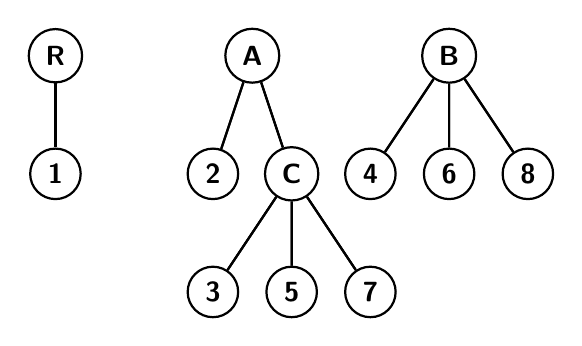
\begin{tikzpicture}[node distance=2.5cm,level distance=1.5cm,
                            level 1/.style={sibling distance=1cm},
                            level 2/.style={sibling distance=1cm},
                            thick,main node/.style={circle,draw,font=\sffamily\bfseries}]

        % Define vertices
        \node[main node] (R) {R}
            child {node[main node] (1) {1}};
        \node[main node] (A) [right of=R] {A}
            child {node[main node] (2) {2}}
            child {node[main node] (C) {C}
                child {node[main node] (3) {3}}
                child {node[main node] (5) {5}}
                child {node[main node] (7) {7}}
            };
        \node[main node] (B) [right of=A] {B}
            child {node[main node] (4) {4}}
            child {node[main node] (6) {6}}
            child {node[main node] (8) {8}};


        % Draw edges
        \path[every node/.style={font=\sffamily\small}]
            (R) edge (1)
            (A) edge (2)
            (A) edge (C)
            (B) edge (4)
            (B) edge (6)
            (B) edge (8)
            (C) edge (3)
            (C) edge (5)
            (C) edge (7);
        \end{tikzpicture}
        \caption{SCC Tree of Graph \ref{fig:graph1} after updates}
        \label{fig:scc_tree_graph_after_del}
    \end{subfigure}
    \caption{SCC Tree updates are propogated, deleting edge 4 to 1}
    \label{fig:scc_tree_after_update_propogation}
\end{figure}


\begin{figure}[H]
    \centering
    \begin{subfigure}{0.45\textwidth}
        \centering
        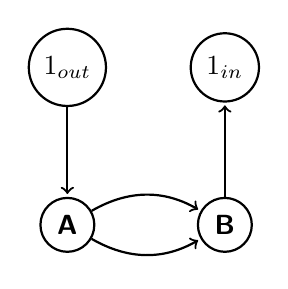
\begin{tikzpicture}[->,shorten >=1pt,auto,node distance=2cm,
            thick,main node/.style={circle,draw,font=\sffamily\bfseries}]

        % Define vertices
        \node[main node] (1) {$1_{in}$};
        \node[main node] (11) [left of=1] {$1_{out}$};
        \node[main node] (A) [below of=11] {A};
        \node[main node] (B) [below of=1] {B};
        

        % Draw edges
        \path[every node/.style={font=\sffamily\small}]
            (11) edge (A)
            (A) edge[bend left] (B)
            (A) edge[bend right] (B)
            (B) edge (1);

        \end{tikzpicture}
        \caption{Graph in SCC Tree Node R}
    \end{subfigure}
    \hfill
    \begin{subfigure}{0.45\textwidth}
        \centering
        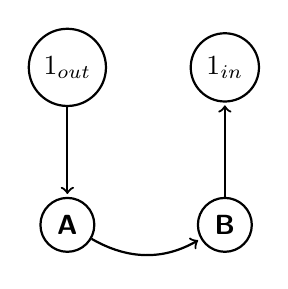
\begin{tikzpicture}[->,shorten >=1pt,auto,node distance=2cm,
            thick,main node/.style={circle,draw,font=\sffamily\bfseries}]

        % Define vertices
        \node[main node] (1) {$1_{in}$};
        \node[main node] (11) [left of=1] {$1_{out}$};
        \node[main node] (A) [below of=11] {A};
        \node[main node] (B) [below of=1] {B};
        

        % Draw edges
        \path[every node/.style={font=\sffamily\small}]
            (11) edge (A)
            (A) edge[bend right] (B)
            (B) edge (1);

        \end{tikzpicture}
        \caption{Graph after deleting edge 3 to 8}
        \label{fig:graph_after_dedge_3_to_8}
    \end{subfigure}
    \caption{Graph in SCC Tree Node R after deleting edge 3 to 8}
    \label{fig:tree_node_r_graph_after_dedge2}
\end{figure}
\subsubsection{Deleting Edge from an Internal Node}\label{Subsubsec: Deleting Edge from an Internal Node}

In this example, we consider the case when the deleted edge (u, v) belongs to an internal node of the SCC tree.
The edge (4, 8) is deleted from the graph held in \textsc{STN}(B), since the lowest common ancestor of 4 and 8 is B from the SCC tree in \figureref{\ref{fig:scc_tree_graph1}}.
We can see in \figureref{\ref{fig:tree_node_b_graph_after_dedge1}} that after removing the edge (4, 8) from the graph in \textsc{STN}(B), vertices 6 and 8 become unreachable from 4.


\begin{figure}[H]
    \centering
    \begin{subfigure}{0.45\textwidth}
        \centering
        \begin{tikzpicture}[->,shorten >=1pt,auto,node distance=2cm,
            thick,main node/.style={font=\sffamily\large\bfseries}]

        % Define vertices
        \node[main node] (4) {$4_{in}$};
        \node[main node] (44) [left of=1] {$4_{out}$};
        \node[main node] (6) [below of=1] {6};
        \node[main node] (8) [below of=11] {8};
        

        % Draw edges
        \path[every node/.style={font=\sffamily\small}]
            (44) edge (8)
            (8) edge (6)
            (6) edge (4);

        \end{tikzpicture}
        \caption{Graph in Tree Node B}
        \label{fig:tree_node_b_graph}
    \end{subfigure}
    \hfill
    \begin{subfigure}{0.45\textwidth}
        \centering
        \begin{tikzpicture}[->,shorten >=1pt,auto,node distance=2cm,
            thick,main node/.style={font=\sffamily\large\bfseries}]

        % Define vertices
        \node[main node] (4) {$4_{in}$};
        \node[main node] (44) [left of=1] {$4_{out}$};
        \node[main node] (6) [below of=1] {6};
        \node[main node] (8) [below of=11] {8};
        

        % Draw edges
        \path[every node/.style={font=\sffamily\small}]
            (8) edge (6)
            (6) edge (4);

        \end{tikzpicture}
        \caption{Graph after deleting edge 4 to 8}
        \label{fig:graph_after_dedge_4_to_8}
    \end{subfigure}
    \caption{Graph in Tree Node B after deleting edge 4 to 8}
    \label{fig:tree_node_b_graph_after_dedge1}
\end{figure}

Since, vertices 6 and 8 are unreachable from 4, we expose these vertices and the corresponding edges in \textsc{STN}(B) to its parent node R.
As shown in \figureref{\ref{fig:tree_node_r_graph_exposed1}}, the unreachable nodes 6 and 8 are exposed to the parent node R by adding edges (8,6), (6,4) from $B$ and
changing the edges (A,B), (B, $1_{in}$) in $R$ to (A,8), (4, $1_{in}$) respectively. The red line in \figureref{\ref{fig:tree_node_r_graph_exposed1}} shows the exposed graph
which was initially a part of $B$.

\begin{figure}[H]
    \centering
    \begin{subfigure}{0.45\textwidth}
        \centering
        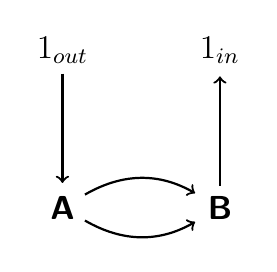
\begin{tikzpicture}[->,shorten >=1pt,auto,node distance=2cm,
            thick,main node/.style={font=\sffamily\large\bfseries}]

        % Define vertices
        \node[main node] (1) {$1_{in}$};
        \node[main node] (11) [left of=1] {$1_{out}$};
        \node[main node] (A) [below of=11] {A};
        \node[main node] (B) [below of=1] {B};
        

        % Draw edges
        \path[every node/.style={font=\sffamily\small}]
            (11) edge (A)
            (A) edge[bend left] (B)
            (A) edge[bend right] (B)
            (B) edge (1);

        \end{tikzpicture}
        \caption{Graph in SCC Tree Node R}
    \end{subfigure}
    \hfill
    \begin{subfigure}{0.45\textwidth}
        \centering
        \begin{tikzpicture}[->,shorten >=1pt,auto,node distance=2cm,
            thick,main node/.style={font=\sffamily\large\bfseries}]

        % Define vertices
        \node[main node] (1) {$1_{in}$};
        \node[main node] (11) [left of=1] {$1_{out}$};
        \node[main node] (A) [below left of=11] {A};
        \node[main node] (8) [below right of=A] {8};
        \node[main node] (6) [right of=8] {6};
        \node[main node] (4) [above right of=6] {4};
        

        % Draw edges
        \path[every node/.style={font=\sffamily\small}]
            (11) edge (A)
            (A) edge[bend left] (8)
            (A) edge[bend right] (8)
            (8) edge (6)
            (6) edge (4)
            (4) edge (1);

        \draw [red, rounded corners, dashed] ($(8) + (-0.5 , 0.5)$) -- ($(6) + (0,0.5)$) -- ($(4) + (-0.5, 0)$) -- ($(4) + (-0.5, 0.5)$) -- ($(4) + (0, 0.5)$) -- ($(4) + (0.5, 0.5)$) -- ($(4) + (0.5, 0)$) 
        -- ($(4) + (0.5, -0.25)$) -- ($(6) + (0.25, -0.5)$) -- ($(8) + (-0.5, -0.5)$) -- cycle;
        \end{tikzpicture}
        \caption{After Exposure}
        \label{fig:tree_node_r_graph_exposed1}
    \end{subfigure}
    \caption{Graph in SCC Tree Node R after unreachable nodes and its corresponding edges are exposed}
\end{figure}

We observe that every vertex in \figureref{\ref{fig:tree_node_r_graph_exposed1}} is reachable, thereby concluding the algorithm.
The above edge and vertex exposure process has a change in the SCC-tree, which is shown in \figureref{\ref{fig:scc_tree_after_update_propogation2}}.

\begin{figure}[H]
\centering
\begin{subfigure}{0.45\textwidth}
    \centering
    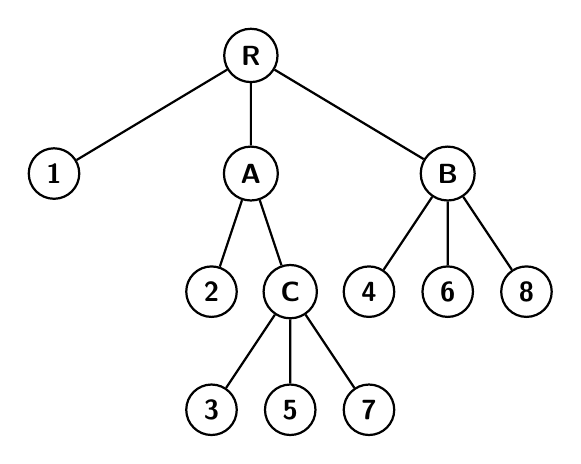
\begin{tikzpicture}[level distance=1.5cm,
                        level 1/.style={sibling distance=2.5cm},
                        level 2/.style={sibling distance=1cm},
                        thick,main node/.style={circle,draw,font=\sffamily\bfseries}]

    % Define vertices
    \node[main node] (R) {R}
        child {node[main node] (1) {1}}
        child {node[main node] (A) {A}
        child {node[main node] (2) {2}}
        child {node[main node] (C) {C}
            child {node[main node] (3) {3}}
            child {node[main node] (5) {5}}
            child {node[main node] (7) {7}}
        }
        }
        child {node[main node] (B) {B}
        child {node[main node] (4) {4}}
        child {node[main node] (6) {6}}
        child {node[main node] (8) {8}}
        };

    \end{tikzpicture}
    \caption{SCC Tree of Graph \ref{fig:graph1}}
\end{subfigure}
\hfill
\begin{subfigure}{0.45\textwidth}
    \centering
    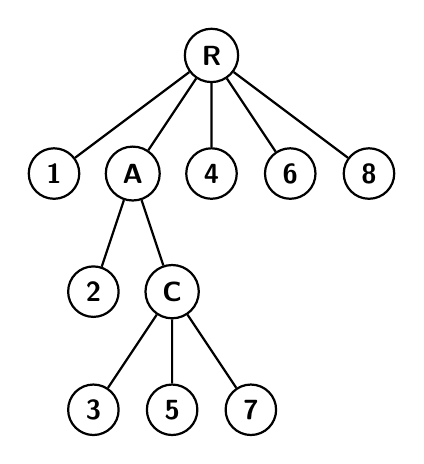
\begin{tikzpicture}[node distance=3cm,level distance=1.5cm,
                        level 1/.style={sibling distance=1cm},
                        level 2/.style={sibling distance=1cm},
                        thick,main node/.style={circle,draw,font=\sffamily\bfseries}]

    % Define vertices
    \node[main node] (R) {R}
        child {node[main node] (1) {1}}
        child {node[main node] (A) {A}
        child {node[main node] (2) {2}}
        child {node[main node] (C) {C}
        child {node[main node] (3) {3}}
        child {node[main node] (5) {5}}
        child {node[main node] (7) {7}}
        }
        }
        child {node[main node] (4) {4}}
        child {node[main node] (6) {6}}
        child {node[main node] (8) {8}}
        ;

    \end{tikzpicture}
    \caption{SCC Tree of Graph \ref{fig:graph1} after updates}
\end{subfigure}
\caption{Tree updates are propogated, deleting edge 4 to 8}
\label{fig:scc_tree_after_update_propogation2}
\end{figure}


\subsection{Incremental Maintaince of SCC Tree}\label{Subsec: Incremental Maintaince of SCC Tree}

In this section, we understand the process of maintaining the SCC tree under the add operation. The \textsc{Add}(u, v) operation introduces the edge from vertex $u$ to vertex $v$ in the graph $G$.
This operation when performed may join strongly connected components or change the internal connectivity of the SCC tree.

\begin{algorithm}[H]
    \SetAlgoLined
    \KwData{G, u, v}
    \KwResult{G'}
    $L = \text{\textsc{LCA}}(u, v)$\;
    $\text{\textsc{STN}}(L).E = \text{\textsc{STN}}(L).E \cup \{(u, v)\}$\;
    \textsc{UpdateSCCTreeI}(L)\;
    \caption{\textsc{Add}(G, u, v)}
\end{algorithm}

For graph $G$ and an edge $(u, v)$ is to be added to the graph $G$. Suppose if the vertex $u$ and $v$ belong to different strongly connected component, 
then the addition of the edge $(u, v)$ might combine multiple SCCs to form a sigle larger SCC. In this case, we add the edge $(u, v)$ to the master node
and update the SCC mapping array to reflect the newly formed SCC. A new SCC-tree node is introduced by adding the vertices and their corresponding edges which were a part of the SCCs that were combined in the master node.
These combined SCCs become the children of the newly formed SCC-tree node. This new SCC-tree node has to propogate its updates to maintain the internal connectivity of the vertices.

However, if the vertices $u$ and $v$ belong to the same strongly connected component, then the addition of the edge $(u, v)$ will never introduce any new SCCs, but would significantly change the internal structuring of the SCC tree.
These changes are to be propogated to maintain the SCC-tree structure and property.
The update propogation is nothing but re-running the SCC-tree creation algorithm on the SCC-tree node that has changes to propogate. The difference is that we do not have to re-run the algorithm on the entire graph, but only on the graphs stored in the SCC-tree nodes.

\begin{algorithm}[H]
    \SetAlgoLined
    \KwData{L | SCC Tree Node}
    \KwResult{Updated SCC Tree}
    $G = \textsc{STN}(L)$, $U = \text{\textsc{FindScc}}(G)$\;
    \For {$U_i \in U$ \textbf{and} $|U_i| \neq 1$} {
        $L_i = \textsc{Label}(U_i)$\;
        $\textsc{STN}(L_i) = \textsc{STN}(L) \cap U_i$\;
        $\textsc{STN}(L_i) = \textsc{Split}(\textsc{STN}(L_i), d)$\;
        $\textsc{UpdateSCCTreeI}(L_i)$\;
    }
    $\textsc{STN}(L) = \textsc{Condense}(G)$\;
    \For {$U_i \in U$ \textbf{and} $|U_i| = 1$} {
        $T = U_i$\;
        \While {$T \neq \emptyset$} {
            $V = T.pop()$\;
            \If {$\textsc{STN}(V).E == \emptyset$} {
                $\textsc{SM}_G(V) = L_i$\;
                \textbf{continue}\;
            }
            $T = T \cup \textsc{STN}(V).V$\;
        }
    }


    \caption{\textsc{UpdateSCCTreeI}(L)}
\end{algorithm}

\subsubsection{Updating SCC-tree under the Add operation}\label{Subsubsec: Updating SCC-tree under the Add operation}

We would now understand the process of updating the SCC-tree, when the edge $(u, v)$ is added to the graph $G$.
The graph in \figureref{\ref{fig:graph2}} is considered for this example, we can observe the SCC-tree of the graph in \figureref{\ref{fig:scc_tree2}}.
The graph has 3 stongly connected components which are identified by labels $R$, $5$ and $7$. 

\begin{figure}[H]
    \centering
    \begin{subfigure}{0.45\textwidth}
        \centering
        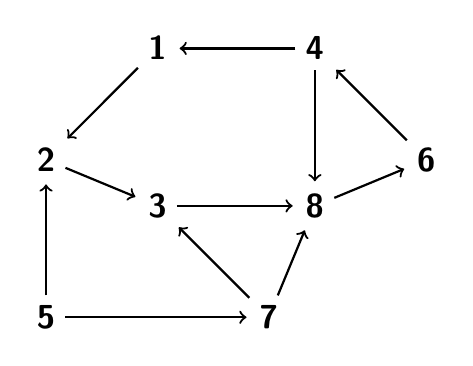
\begin{tikzpicture}[->,shorten >=1pt,auto,node distance=2cm,
                            thick,main node/.style={font=\sffamily\large\bfseries}]

        % Define vertices
        \node[main node] (1) {1};
        \node[main node] (2) [below left of=1] {2};
        \node[main node] (3) [below of=1] {3};
        \node[main node] (4) [right of=1] {4};
        \node[main node] (5) [below left of=3] {5};
        \node[main node] (6) [below right of=4] {6};
        \node[main node] (7) [below right of=3] {7};
        \node[main node] (8) [right of=3] {8};

        % Draw edges
        \path[every node/.style={font=\sffamily\small}]
            (1) edge (2)
            (2) edge (3)
            (3) edge (8)
            (4) edge (1)
            (4) edge (8)
            (5) edge (2)
            (5) edge (7)
            (6) edge (4)
            (7) edge (3)
            (7) edge (8)
            (8) edge (6);

        \end{tikzpicture}
        \caption{Graph 2}
        \label{fig:graph2}
    \end{subfigure}
    \begin{subfigure}{0.45\textwidth}
        \centering
        \begin{tikzpicture}[level distance=1.5cm,
                            level 1/.style={sibling distance=1.25cm},
                            level 2/.style={sibling distance=1cm},
                            thick,main node/.style={circle,draw,font=\sffamily\bfseries}]

        % Define vertices
        \node[main node] (R) {R}
            child {node[main node] (1) {1}}
            child {node[main node] (2) {2}}
            child {node[main node] (3) {3}}
            child {node[main node] (B) {B}
                child {node[main node] (4) {4}}
                child {node[main node] (6) {6}}
                child {node[main node] (8) {8}}
            };
        \node[main node, right=1.5cm of R] (5) {5};
        \node[main node, right=1.25cm of 5] (7) {7};
        \end{tikzpicture}

        \caption{SCC Tree of Graph 2} 
        \label{fig:scc_tree2}      
    \end{subfigure}
    \caption{Graph 2 and its SCC-trees}
    \label{fig:graph2_scc_tree}
\end{figure}
 

The edge $(3,5)$ is added to the graph, it combines the strongly connected components $R$, $5$ and $7$ to form a single SCC $R'$.
This change can be seen in the figure \figureref{\ref{fig:graph2_condense}}, we notice that the edge (3,5) correponds to the edge (R',5)
in the master node, which upon addtion combines the SCCs $R$, $5$ and $7$.

\begin{figure}[H]
    \centering
    \begin{subfigure}{0.4\textwidth}
        \centering
        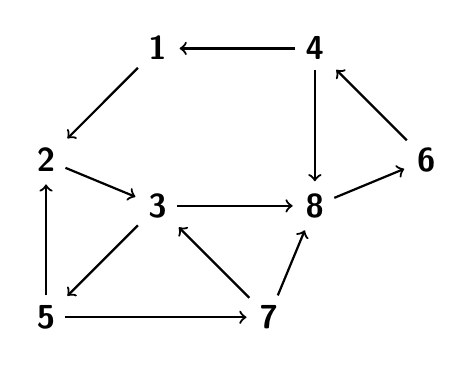
\begin{tikzpicture}[->,shorten >=1pt,auto,node distance=2cm,
                            thick,main node/.style={font=\sffamily\large\bfseries}]

        % Define vertices
        \node[main node] (1) {1};
        \node[main node] (2) [below left of=1] {2};
        \node[main node] (3) [below of=1] {3};
        \node[main node] (4) [right of=1] {4};
        \node[main node] (5) [below left of=3] {5};
        \node[main node] (6) [below right of=4] {6};
        \node[main node] (7) [below right of=3] {7};
        \node[main node] (8) [right of=3] {8};

        % Draw edges
        \path[every node/.style={font=\sffamily\small}]
            (1) edge (2)
            (2) edge (3)
            (3) edge (8)
            (4) edge (1)
            (4) edge (8)
            (5) edge (2)
            (5) edge (7)
            (6) edge (4)
            (7) edge (3)
            (7) edge (8)
            (8) edge (6)
            (3) edge (5);

        \end{tikzpicture}
        \caption{Graph 2}
    \end{subfigure}
    \begin{subfigure}{0.3\textwidth}
        \centering
        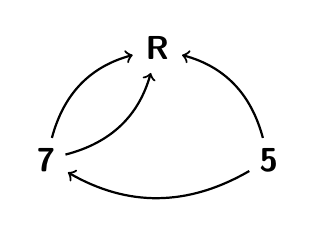
\begin{tikzpicture}[->,shorten >=1pt,auto,node distance=2cm,
                            thick,main node/.style={font=\sffamily\large\bfseries}]

        % Define vertices
        \node[main node] (R) {R};
        \node[main node] (5) [below right of=R] {5};
        \node[main node] (7) [below left of=R] {7};

        % Draw edges
        \path[every node/.style={font=\sffamily\small}]
            (5) edge[bend right] (R)
            (5) edge[bend left] (7)
            (7) edge[bend right] (R)
            (7) edge[bend left] (R);

        \end{tikzpicture}
        \caption{\textsc{Condense}(G) before \textsc{Add}}
        \label{fig:condense_before_add}      
    \end{subfigure}
    \begin{subfigure}{0.3\textwidth}
        \centering
        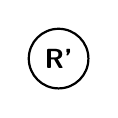
\begin{tikzpicture}[->,shorten >=1pt,auto,node distance=2cm,
                            thick,main node/.style={draw,circle,font=\sffamily\bfseries}]

        % Define vertices
        \node[main node] (R') {R'};

        \end{tikzpicture}
        \caption{\textsc{Condense}(G) after \textsc{Add}}
        \label{fig:condense_after_add}
    \end{subfigure}
    \caption{Graph 2, \textsc{Condense}(G) before and after \textsc{Add}}
    \label{fig:graph2_condense}
\end{figure}
 

A new SCC-tree node $R'$ is introduced to represent the new SCC formed by the addition of the edge $(3,5)$.
It captures the subgraph that is formed by the vertices and edges that were a part of the SCCs $R$, $5$ and $7$.
The SCC-tree node $R'$ graph is split on the vertex $7$, as shown in \figureref{\ref{fig:stn_r_before_after_split}}.
When we condense the graph in \textsc{STN}(R'), we find that the vertices $R$ and $5$ combine to form a single vertex $A$, as shown in \figureref{\ref{fig:stn_a_and_updated_scc_tree}}.

\begin{figure}[H]
    \centering
    \begin{subfigure}{0.3\textwidth}
        \centering
        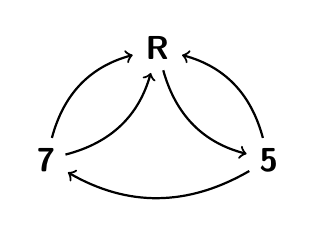
\begin{tikzpicture}[->,shorten >=1pt,auto,node distance=2cm,
                            thick,main node/.style={font=\sffamily\large\bfseries}]

        % Define vertices
        \node[main node] (R) {R};
        \node[main node] (5) [below right of=R] {5};
        \node[main node] (7) [below left of=R] {7};

        % Draw edges
        \path[every node/.style={font=\sffamily\small}]
            (5) edge[bend right] (R)
            (5) edge[bend left] (7)
            (7) edge[bend right] (R)
            (7) edge[bend left] (R)
            (R) edge[bend right] (5);

        \end{tikzpicture}
        \caption{\textsc{STN}(R') before \textsc{Split}}
    \end{subfigure}
    \begin{subfigure}{0.3\textwidth}
        \centering
        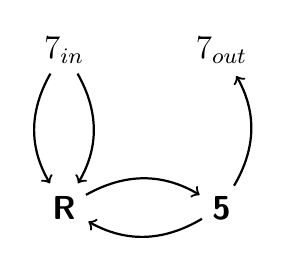
\begin{tikzpicture}[->,shorten >=1pt,auto,node distance=2cm,
                            thick,main node/.style={font=\sffamily\large\bfseries}]

        % Define vertices
        \node[main node] (7) {$7_{in}$};
        \node[main node] (77) [right of=7] {$7_{out}$};
        \node[main node] (5) [below of=77] {5};
        \node[main node] (R) [below of=7] {R};

        % Draw edges
        \path[every node/.style={font=\sffamily\small}]
            (7) edge[bend right] (R)
            (7) edge[bend left] (R)
            (5) edge[bend right] (77)
            (5) edge[bend left] (R)
            (R) edge[bend left] (5);

        \end{tikzpicture}
        \caption{\textsc{STN}(R') after \textsc{Split}}
    \end{subfigure}
    \begin{subfigure}{0.3\textwidth}
        \centering
        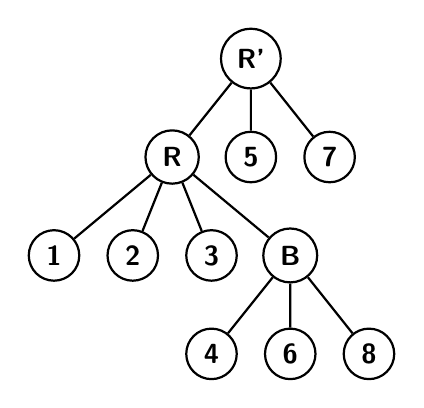
\begin{tikzpicture}[level distance=1.25cm,
                            level 1/.style={sibling distance=1cm},
                            level 2/.style={sibling distance=1cm},
                            thick,main node/.style={circle,draw,font=\sffamily\bfseries}]

        % Define vertices
        \node[main node] (R') {R'}
            child {node[main node] (R) {R}
                child {node[main node] (1) {1}}
                child {node[main node] (2) {2}}
                child {node[main node] (3) {3}}
                child {node[main node] (B) {B}
                    child {node[main node] (4) {4}}
                    child {node[main node] (6) {6}}
                    child {node[main node] (8) {8}}
                }
            }
            child {node[main node] (5) {5}}
            child {node[main node] (7) {7}};
        \end{tikzpicture}

        \caption{updated SCC-tree}     
    \end{subfigure}
    \caption{\textsc{STN}(R') before and after \textsc{Split} and updated SCC-tree}
    \label{fig:stn_r_before_after_split}
\end{figure}
 

The new SCC-tree node $A$ is introduced that captures the subgraph formed by the vertices and edges that were a part of $R$ and $5$, in the SCC-tree node $R'$. 
This graph can be seen in \figureref{\ref{fig:stn_a_and_updated_scc_tree}}, when we condense the graph in \textsc{STN}(A), we find that no combination of vertices is possible, and thus the SCC-tree is updated.
The SCC-tree is updated to reflect changes brought by the addition of the edge $(3,5)$ is shown in \figureref{\ref{fig:stn_a_and_updated_scc_tree}}.

\begin{figure}[H]
    \centering
    \begin{subfigure}{0.3\textwidth}
        \centering
        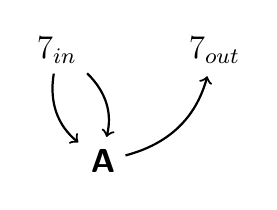
\begin{tikzpicture}[->,shorten >=1pt,auto,node distance=2cm,
                            thick,main node/.style={font=\sffamily\large\bfseries}]

        % Define vertices
        \node[main node] (7) {$7_{in}$};
        \node[main node] (77) [right of=7] {$7_{out}$};
        \node[main node] (A) [below left of=77] {A};

        % Draw edges
        \path[every node/.style={font=\sffamily\small}]
            (7) edge[bend right] (A)
            (7) edge[bend left] (A)
            (A) edge[bend right] (77);

        \end{tikzpicture}
        \caption{\textsc{STN}(R') after \textsc{Condense}}
    \end{subfigure}
    \begin{subfigure}{0.3\textwidth}
        \centering
        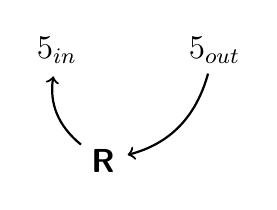
\begin{tikzpicture}[->,shorten >=1pt,auto,node distance=2cm,
                            thick,main node/.style={font=\sffamily\large\bfseries}]

        \node[main node] (5) {$5_{in}$};
        \node[main node] (55) [right of=5] {$5_{out}$};
        \node[main node] (R) [below left of=55] {R};

        \path[every node/.style={font=\sffamily\small}]
            (55) edge[bend left] (R)
            (R) edge[bend left] (5);

        \end{tikzpicture}
        \caption{\textsc{STN}(A)}
    \end{subfigure}
    \begin{subfigure}{0.3\textwidth}
        \centering
        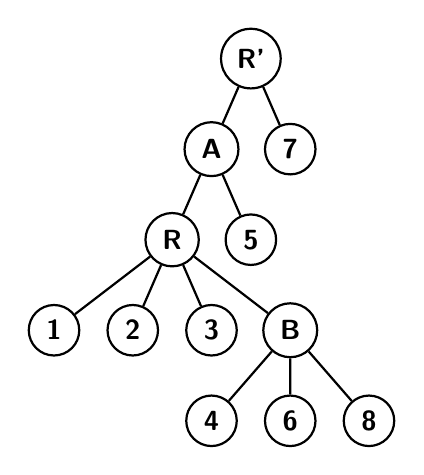
\begin{tikzpicture}[level distance=1.15cm,
                            level 1/.style={sibling distance=1cm},
                            level 2/.style={sibling distance=1cm},
                            thick,main node/.style={circle,draw,font=\sffamily\bfseries}]

        % Define vertices
        \node[main node] (R') {R'}
            child {node[main node] (A) {A}
                child {node[main node] (R) {R}
                    child {node[main node] (1) {1}}
                    child {node[main node] (2) {2}}
                    child {node[main node] (3) {3}}
                    child {node[main node] (B) {B}
                        child {node[main node] (4) {4}}
                        child {node[main node] (6) {6}}
                        child {node[main node] (8) {8}}
                    }
                }
                child {node[main node] (5) {5}}
            }
            child {node[main node] (7) {7}};
        \end{tikzpicture}

        \caption{updated SCC-tree}     
    \end{subfigure}
    \caption{\textsc{STN}(R'), \textsc{STN}(A) and updated SCC-tree}
    \label{fig:stn_a_and_updated_scc_tree}
\end{figure}
 



\section{Practical Implementation} \label{Sec: Practical Implementation}

In this part, we delve into the practical implementation of our algorithm for maintaining strongly connected components (SCCs) within large-scale graphs using MPI in C++. 
By leveraging MPI's robust framework, we endeavor to unlock the full potential of parallelism, distributing the computational load across multiple nodes to expedite the identification and maintenance of SCCs.

Message Passing Interface (\hyperref[mpi]{MPI}), is a standardized and portable message-passing system designed to facilitate parallel computing across a distributed memory system.
In the further sections, we will discuss the data structures used, the workload distribution in parallel, and the cache optimizations that were implemented to enhance the performance of our algorithm.

We will be using the Boost MPI library for the implementation of the algorithm. The Boost MPI library provides a high-level interface for the Message Passing Interface (MPI) standard, enabling the development of parallel applications in C++.
We would also be using the Boost Serialization library for serializing the data structures used in the algorithm. This library provides a framework for serializing and deserializing C++ data structures to and from a sequence of bytes, facilitating the transmission of data across a network.

\subsection{Data Structures}\label{Subsec: Data Structures}
In distributed parallel computing, the efficacy of algorithms often hinges upon the efficiency of their underlying data structures. 
In this section, we discuss the design and characteristics of the data structures introduced in the theoretical underpinnings of our SCC maintenance algorithm.
By elucidating their intricacies, time complexities, and other pertinent aspects, we aim to provide a comprehensive understanding of their role in facilitating efficient graph analysis within a distributed computing environment.

\subsubsection{SCC Tree}\label{Subsubsec: SCC Tree DS}
The SCC-tree introduced in \secref{\ref{Subsubsec: SCC Tree}} is a hierarchical data structure that encapsulates the SCCs within a directed graph.
It comprises of various components, including the SCC-tree node, the SCC-tree edge, and the SCC-tree itself.

The Edge class is a simple data structure that encapsulates the source and destination vertices of an edge within the graph stored in a SCC-tree node.
The serialization and equality operator overloads are implemented to facilitate the serialization of the Edge object and comparison of two Edge objects.
The Edge class is defined in Lst.\ref{lst:edge}.

\begin{lstlisting}[language=C++, caption={Edge}, label={lst:edge}]
class Edge {
public:
    long int from;
    long int to;

    Edge() {}
    Edge(int from , int to) : from(from), to(to) {}

    friend boost::serialization::access;
    template < class Archive >
    void serialize(Archive & ar, const unsigned int version) {
        ar & from;
        ar & to;
    }

    bool operator==(const Edge& other) const {
        return from == other.from && to == other.to;
    }
};
\end{lstlisting}

The SCC-tree node class encapsulates vertices and edges connecting them, forming a graph, as discussed in \secref{\ref{Subsubsec: SCC Tree}}.
The class comprises various components, including the label, parent, corresponds-to, contains, and dept, which are described in detail in Lst.\ref{lst:scc_tree_node}.
The SCC-tree node class also includes various functions, such as condenseFill, checkUnreachable, updateLabels, exposeToParent, and removeEdge, which are used to manipulate the SCC-tree node and its components.

\begin{lstlisting}[language=C++, caption={SCC-Tree Node}, label={lst:scc_tree_node}]
class TreeNode {
public:
    /**
        * @brief this would represent the label of the node in the SCC tree
        * the label is unique for each node in the SCC tree
        * 
        */
    long int                            label;
    /**
        * @brief this represents the parent of the current node in the SCC tree
        *  and is used to traverse the tree upwords.
        * 
        */
    long int                            parent;
    /**
        * @brief stores the actual edge to labelled edge pair,
        * nodes forming a scc are condesed to one labelled node, and so are the edges,
        * the corresponds_to is used to store the actual edges to labelled edges
        * relationship.
        * 
        */
    std::vector<std::pair<Edge, Edge>>  corresponds_to;
    /**
        * @brief contains the nodes which are part of the current node in the SCC tree.
        * They store the label of the child nodes and is used to travese the tree 
        * downwards.
        * 
        */
    std::unordered_set<long int>        contains;
    /**
        * @brief stores the depth of the current node in the SCC tree and is
        * used to find the LCA of two nodes (Lowest Common Ancestor), 
        * important for update operations.
        * 
        */
    long int                            dept;
    /**
        * @brief The following function is used to serialize the TreeNode object,
        * this is essential for the boost::serialization to work. The TreeNodes are 
        * transferred during update queries.
        * 
        */
    friend                              boost::serialization::access;
    template < class Archive >
    void serialize(Archive & ar, const unsigned int version) {
        ar & label;
        ar & parent;
        ar & corresponds_to;
        ar & contains;
        ar & dept;
    }

    /**
        * @brief the function is used to fill the corresponds_to edge pairs for the 
        * current node.The sccs is used to find the labelling of the nodes in the 
        * graph and create the corresponding edges in the SCC tree.
        * 
        * @param edges are the actual edge present in the graph
        * @param sccs is a unordered_map which stores the nodes and their 
        * corresponding sccs to which they belong.
        */
    void condenseFill(std::vector<Edge>& edges, 
                std::unordered_map<long int, long int>& sccs);
    /**
        * @brief the function is used to find the unreachable nodes in the current node.
        * 
        * @param unreachable is a set which stores the unreachable nodes after its 
        * execution.
        */
    void checkUnreachable(std::unordered_set<long int>& unreachable);
    /**
        * @brief the function is used to update the labels of the nodes in the 
        * current node.
        * 
        * @param new_labels is a unordered_map which stores the new labels of the nodes.
        */
    void updateLabels(std::unordered_map<long int, long int>& new_labels);
    /**
        * @brief the function is used to indentify the edges which are unreachable 
        * in the current node, and transfer them to the parent by appropriately updating
        * their labels and adding them to the parent node.
        * 
        * @param parent The parent node to which the unreachable edges are to be 
        * transferred
        * @param unreachable Set of unreachable nodes in the current node
        */
    void exposeToParent(TreeNode& parent, std::unordered_set<long int> unreachable);
    /**
        * @brief the function is used to remove the edge from the current node.
        * 
        * @param edge The edge to be removed from the current node
        */
    void removeEdge(const Edge& edge);

    //copy constructor
    TreeNode(const TreeNode& other) {
        label = other.label;
        parent = other.parent;
        corresponds_to = other.corresponds_to;
        contains = other.contains;
        dept = other.dept;
    }
    //assignment operator
    TreeNode& operator=(const TreeNode& other) {
        label = other.label;
        parent = other.parent;
        corresponds_to = other.corresponds_to;
        contains = other.contains;
        dept = other.dept;
        return *this;
    }
    //default constructor
    TreeNode() {
        label = -1;
        parent = -1;
        dept = 0;
    }
};
\end{lstlisting}

The SCC-tree is collection of SCC-tree nodes, forming a tree structure that encapsulates the SCCs within a directed graph.
This information is stored in the form of mappings between the labels of the nodes and the corresponding SCC-tree nodes.
We hold the labels of the root nodes of the SCC-tree in a vector, which is used to traverse the tree and perform various operations.

\begin{lstlisting}[language=C++, label={lst:scc_tree}]
    std::vector<long int> root_nodes;
    std::unordered_map<long int, TreeNode> scc_tree_nodes;
\end{lstlisting}

\subsubsection{SCC Mapping Array}\label{Subsubsec: SCC Mapping Array DS}
The SCC mapping array is a data structure that would store the mapping of the vertices to the SCCs label they belong to.
We use an unordered map to store this information as it provides an average time complexity of O(1) for insertion, deletion, and lookup operations.
\begin{lstlisting}[language=C++, label={lst:scc_mapping_array}]
    std::unordered_map<long int, long int> scc_mapping;
\end{lstlisting}

\subsection{Workload Distribution in Parallel}\label{Subsec: Workload Distribution in Parallel}
In this section, we discuss how the workload is distributed across multiple nodes in a parallel computing environment using MPI.
The algorithm is designed to distribute the graph data across multiple nodes, with each node responsible for processing them separately.
In future references, we will refer to these nodes as cores or processors interchangeably. Every core is assigned a unique rank, which is used to identify them in the MPI environment.
These cores would each be reposible for storing an instance of class \textit{MaintainSCC}, which would contain nessary data structures and functions to perform the SCC maintenance operations.

The \textit{MaintainSCC} class contains the following:
\begin{itemize}
    \item \textsc{SCC\_LABEL}: A unique label that is assigned, if we form a new SCC-tree node. It is an integer corresponding to the next available (unused) label.
    \item world\_size: The total number of cores in the MPI environment, used to assigned workload.
    \item roots: A vector that stores the labels of the root nodes of the SCC-tree.
    \item scc\_tree\_nodes: A map that stores the mapping between the labels of the nodes and the corresponding SCC-tree nodes.
    \item delete\_cache: A set that stores the nodes that were affected by the deletion of edges.
    \item insert\_cache: A set that stores the nodes that were affected by the insertion of edges.
    \item rank: A map that stores a mapping between each vertex in the graph and the rank of the core that is responsible for it. In other words, it stores the rank of the core that contains the vertex.
    \item scc\_mapping: A map that stores the mapping between the vertices and the SCCs they belong to.
\end{itemize}

Since, MPI is a message passing interface, we need to define the message types that would be used to communicate between the cores. The following message types are defined:
\begin{itemize}
    \item SCC\_TREE: Used to transfer data that is used in the creation of SCC-tree.
    \item EDGE\_DELETE: Used to transfer the edges that need to be deleted between the cores.
    \item EDGE\_INSERT: Used to transfer the edges that need to be inserted between the cores.
    \item EDGE\_QUERY: Used to transfer the edges that need to be queried between the cores.
    \item SCC\_TRANSFER: Used to transfer the SCC-tree for load balancing.
    \item CLR\_DEC\_CACHE: Used to clear the delete cache.
    \item CLR\_INC\_CACHE: Used to clear the insert cache.
    \item EXIT: Used to signal the end of the program.
\end{itemize}

\begin{lstlisting}[language=C++, label={lst:workload_distribution}]
class MaintainSCC {

    long int                                SCC_LABEL = 0;
    const long int                          MOD = 1e10;
    int                                     world_size;
    std::vector<long int>                   roots;
    std::unordered_map<long int, TreeNode>  scc_tree_nodes;
    std::set<Cache, DecCache>               delete_cache;
    std::set<Cache, IncCache>               insert_cache;
    std::unordered_map<long int, int>       rank;
    std::unordered_map<long int, long int>  scc_mapping;

    enum MessageType
    {
        SCC_TREE,
        EDGE_DELETE,
        EDGE_INSERT,
        EDGE_QUERY,
        SCC_TRANSFER,
        CLR_DEC_CACHE,
        CLR_INC_CACHE,
        EXIT
    };

    /** some internal functions **/
    /**         .......         **/
public:
    bool query(long int v1, long int v2);
    void deleteEdges(std::vector<Edge> &decrement);
    void insertEdges(std::vector<Edge> &increament);
    void endAll();

    MaintainSCC(long int n, std::vector<Edge> &edges);
    ~MaintainSCC();
};
\end{lstlisting}

The 0th core is responsible for the initialization of the graph and the distribution of the workload across the cores.
It takes in the entire graph and runs the SCC algorithm to find the SCCs in the graph, and then distributes the vertices and edges across the cores based on the SCCs they belong to.
The other cores are responsible for constructing the SCC-tree and maintaining the SCCs in the graph, this distribution is stored in the \textit{rank} map. During this process, the 0th core also constructs and maintains the master node and the SCC mapping array.

The other cores work parallelly to construct the SCC-tree in the initialization stage. Once the SCC-tree is constructed, the cores are synchorized and ready for the update queries.
When we call for an update, it is processed in the 0th core, which identifies to which core the update belongs to and sends the same. Upon recieving the update, the core processes the update and sends the result back to the 0th core.
The following situation may arise:
\begin{itemize}
    \item In case of an insert query, two SCCs might get combined to form a new SCC. Here, the master node is updated in the 0th core and upon identifying the 
SCCs that are combined, the SCC-tree corresponding to these components are sent from their respective cores to a common one. This
ensures that the update propogation happens in a synchorized and easier manner.
    \item In case of a delete query, the SCCs might get divided into two or more SCCs. In this case, the labels of the newly created SCCs are sent to the 0th core, which then updates the master node, the SCC mapping array and sends the new label - core mapping back to the updated core.
Upon recieving the new label - core mapping, the current core sends these SCCs to the respective cores, thereby balancing the load.
\end{itemize}

All other functionallity are implemented based on the above mentioned design and algorithm in \secref{\ref{Sec: Theoretical Methodology}}. The public functions in the \textit{MaintainSCC} class are used to interact with the cores and perform the necessary operations.
These functions can only be called from the 0th core, which then analyzes and forwards the request to the respective core.

\subsection{Update Cache Optimizations}\label{Subsec: Cache Optimizations}

In the section, we discuss the cache optimizations that were implemented to enhance the performance of the algorithm.
When we delete or insert an edge in the graph, it affects the structuring of the SCC-tree and hence the changes have to be propogated.
We notice that the process of propogation of changes is time consuming and can be optimized by caching the changes and propogating them in batches.
For understanding the cache optimizations, we need to understand the following, referring to the article \cite{scc_tree_reference}:
\begin{itemize}
    \item An SCC-tree can be constructed in $O(m\delta)$ time, where $\delta$ is the height of
the resulting tree and $m$ is the edges part of that tree. It requires $O(n + m)$ space.
    \item Given an SCC-tree of height $\delta$, the algorithm processes any sequence of
    edge updates in $O(m\delta)$ total time and answers each query in $O(1)$ time, using $O(n + m)$
    space.
\end{itemize}

Given a SCC-tree of height $\delta$, we can delete or insert an edge in $O(\delta)$ time. This is because the deletion or insertion of an edge can affect the SCC-tree in the worst case by $\delta$ levels.
The propogation of changes can be done in $O(m\delta)$ time, thus it is beneficial to cache the changes and propogate them in batches.

Suppose there are $t$ updates to the graph, then the time complexity of the entire process would be $O(tm\delta)$, with the cache optimizations, the time complexity would be $O(m\delta + t\delta)$,
where $t\delta$ is time taken to delete/insert edge only, and $m\delta$ is time taken to propogate changes. The time complexity is reduced from $O(tm\delta)$ to $O((m + t)\delta)$.

\begin{lstlisting}[language=C++, caption={Cache Optimizations}, label={lst:cache_optimizations}]
class Cache {
public:
    long int        dept;
    long int        label;

    bool operator<(const Cache& other) const {
        return dept < other.dept;
    }
    bool operator==(const Cache& other) const {
        return dept == other.dept && label == other.label;
    }
};

class DecCache : public Cache {
public:
    bool operator() (const Cache& a, const Cache& b) const {
        return a.dept > b.dept;
    }
};

class IncCache : public Cache {
public:
    bool operator() (const Cache& a, const Cache& b) const {
        return a.dept < b.dept;
    }
};

std::set<Cache, DecCache>               delete_cache;
std::set<Cache, IncCache>               insert_cache;
\end{lstlisting}

We notice in \secref{\ref{Subsec: Decremental Maintaince of SCC Tree}} and \secref{\ref{Subsec: Incremental Maintaince of SCC Tree}}, 
that for decremental changes we need to propogate the changes from the node to the parent, and for incremental changes we need to propogate the changes from the node to the child node.
Thus, we use two sets, one for decremental changes and one for incremental changes with following properties:
\begin{itemize}
    \item The class \textit{Cache} is used to store the label of the node and its depth in the SCC-tree.
    \item The class \textit{DecCache} is used to define sorting order for the decremental cache, where the nodes are sorted in decreasing order of their depth.
Since, we need to propogate the changes from the node to the parent, we need to start from the deepest node and move upwards.
    \item The class \textit{IncCache} is used to define sorting order for the incremental cache, where the nodes are sorted in increasing order of their depth.
Since, we need to propogate the changes from the node to the child node, we need to start from the shallowest node and move downwards.

\end{itemize}

\begin{table}[H]
    \centering
    \caption{Timings with/without Cache Optimizations (\texttt{Amazon0302})}
    \begin{tabular}{|c|c|c|}
        \hline
        \textbf{Updates(\%)} & \textbf{With Caching} & \textbf{Without Caching} \\
        \hline
        0 & 9.04671 & 10.0534 \\
        1.0 & 2.09399 & 15.9024 \\
        5.0 & 2.24362 & 23.2398\\
        10.0 & 2.34654 & 40.28242 \\
        20.0 & 2.6431 & 50.2302 \\
        30.0 & 2.83777 & 56.28420 \\
        50.0 & 3.25233 & 88.23823\\
        \hline
    \end{tabular}
    \label{tab:cache_optimizations}
\end{table}

\subsection{Challenges in Implementation with MPI}\label{Subsec: Challenges in Implementation with MPI}

Utilizing the MPI library in C++ for distributed parallel computing introduces a unique set of challenges that demand careful consideration and adept problem-solving strategies. 
Below, we outline some common challenges encountered during MPI programming and the way we dealt with them:
\begin{itemize}
    \item \textbf{Load Balancing}: One of the primary challenges in distributed computing is ensuring that the workload is evenly distributed across all nodes.
We addressed this issue by distributing the vertices and edges based on the SCCs they belong to, thereby ensuring that each core receives a balanced workload.
Though this approach is effective, it may lead to an imbalance in the workload if the graph is not well-distributed.
We plan to address this issue by implementing load balancing based upon the number of SCC-tree nodes each core is responsible for, in the future iterations of the algorithm.
This would ensure that each core receives an equal number of SCC-tree nodes, thereby balancing the workload.
    \item \textbf{Communication Overhead}: In a distributed computing environment, communication overhead can significantly impact the performance of the algorithm. This is especially true in MPI programming, where inter-process communication is a crucial aspect.
We tried to minimize the communication overhead by reducing the number of messages exchanged between the cores. This was achieved by the work distribution strategy, where the 0th core is responsible for processing the updates and distributing them to the respective cores.
    \item \textbf{Synchronization}: Synchronization is a critical aspect of parallel computing, especially in distributed environments where multiple nodes are involved.
Since, the updates are processed parrallely in the cores, we had to ensure that the cores are synchronized, by using specialized Message Types to signal the end of the program and to synchronize the cores. 
MPI provides various synchronization mechanisms, such as barriers and point-to-point communication, which we leveraged to ensure that the cores are synchronized.
    \item \textbf{SCC-tree transfer}: When an SCC is formed or divided, the SCC-tree corresponding to these SCCs needs to be transferred between the cores.
These transfers can lead to deadlocks if not handled properly, as the cores may be waiting for each other to send the SCC-tree. We addressed this issue by using a two-phase commit protocol, 
where the cores first signal the 0th core about the SCCs that are formed or divided, and then the 0th core sends the SCC-tree to the respective cores.
    \item \textbf{Memory Management and Resource Consumption}:  Inefficient memory utilization and excessive resource consumption can lead to performance degradation and system instability.
The testing server was very much capable of handling the memory requirements of the algorithm, but this might not be the case in a real-world scenario.
The implementation must be optimized to minimize memory consumption and ensure efficient resource utilization, by using memory pooling and other memory management techniques.
    \item \textbf{Debugging and Testing}: Debugging and testing distributed parallel algorithms can be challenging due to the inherent complexity of the system.
We used various debugging tools provided by MPI, such as MPI\_Error\_string and MPI\_Abort, to identify and resolve issues in the code. 
We also employed unit testing and integration testing to ensure that the algorithm functions correctly in a distributed environment.
The testing was done on a local cluster, and the results were compared with the sequential implementation to verify the correctness of the algorithm.
    \item \textbf{Recursion Limit}: The SCC-tree construction algorithm is recursive in nature, which can lead to stack overflow errors if the recursion depth is too high.
We addressed this issue by implementing iterative versions of recursive algorithms where possible to avoid stack overflow issues. 
Alternatively, increase the stack size or switch to non-recursive approaches to mitigate segmentation faults.
\end{itemize}

\section{Results}\label{Sec: Results}
In this section, we present the results of the experiments conducted. The results are in the form of tables and graphs.
The details of the graphs used in the experiments are presented in Table \ref{tab:graph_details}. 
The tables \ref{tab:timed_results_g1} to \ref{tab:timed_results_g8} present the timings for the experiments conducted on the graphs. 
The timings are presented in seconds. The tables present the timings for the decremental, incremental, and both update operations. 
The timings presented, compares the standard static algorithm to the dynamically maintained parallel algorithm. 
The timings are presented for different percentages of updates w.r.t. edges. 

The machine specifications are retrieved using the \texttt{lscpu} command. The machine specifications are as follows:
\begin{description}[font=\sffamily\bfseries\small,itemsep=0pt,parsep=0pt]
    \item[Architecture:] x86\_64
    \item[CPU op-mode(s):] 32-bit, 64-bit
    \item[Byte Order:] Little Endian
    \item[CPU(s):] 80
    \item[On-line CPU(s) list:] 0-79
    \item[Thread(s) per core:] 2
    \item[Core(s) per socket:] 20
    \item[Socket(s):] 2
    \item[NUMA node(s):] 2
    \item[Vendor ID:] GenuineIntel
    \item[CPU family:] 6
    \item[Model:] 85
    \item[Model name:] Intel(R) Xeon(R) Gold 6248 CPU @ 2.50GHz
    \item[Stepping:] 7
    \item[CPU MHz:] 1000.061
    \item[CPU max MHz:] 3900.0000
    \item[CPU min MHz:] 1000.0000
    \item[BogoMIPS:] 5000.00
    \item[Virtualization:] VT-x
    \item[L1d cache:] 32K
    \item[L1i cache:] 32K
    \item[L2 cache:] 1024K
    \item[L3 cache:] 28160K
    \item[NUMA node0 CPU(s):] 0-19,40-59
    \item[NUMA node1 CPU(s):] 20-39,60-79
\end{description}

The software specifications are retrieved using the \texttt{gcc --version}, \texttt{mpirun --version}, \texttt{boost --version}, and \texttt{cmake --version} commands.
The kernel and OS specifications, are retrieved using the \texttt{hostnamectl} command. The above specifications are as follows:
\begin{description}[font=\sffamily\bfseries\small,itemsep=0pt,parsep=0pt]
    \item[Operating System:] Red Hat Enterprise Linux Server 7.6 (Maipo)
    \item[Kernel:] 3.10.0-957.el7.x86\_64
    \item[Compiler:] gcc version 9.2.0
    \item[OpenMPI:] 3.1
    \item[Boost:] 1.84.0
    \item[CMake:] 2.8.12.2
\end{description}

\begin{table}[H]
    \centering
    \caption{Graph Details}
    \begin{tabular}{|c|c|c|}
        \hline
        \textbf{Graph} & \textbf{Number of Vertices} & \textbf{Number of Edges} \\
        \hline
        \texttt{cleancom-orkutud-SCC} & 3,072,441 & 234,370,166 \\
        \texttt{clean-soc-sinaweibo-SCC} & 58,655,849 & 261,321,071 \\
        \texttt{cleanWikipedia-SCC} & 3,370,462 & 93,373,056 \\
        \texttt{livjournal-SCC} & 4,847,571 & 68,993,773 \\
        \texttt{clean-soc-pokec-relationships-SCC} & 1,632,803 & 30,622,564 \\
        \texttt{clean-soc-twitter-SCC} & 21,297,772 & 265,025,809 \\
        \texttt{rmat876-SCC} & 16,777,216 & 87,654,320 \\
        \texttt{u10m\_80m-SCC} & 10,000,000 & 80,000,000 \\
        \hline
    \end{tabular}
    \label{tab:graph_details}
\end{table}

The each graph, the algorithm was tested by increasing the total number of updates w.r.t. the percentage of edges present in the graph. 
The $0$ percent edge updates, indicates the time taken to initialization the SCC-tree for the maintaince process. 
The subsequent tests conducted, reveal the time taken to update the SCC-tree for the given percentage of updates. 
All the testing was conducted on the same machine, with \texttt{-np} parameter set to $64$ for the \texttt{mpirun} command.


\begin{table}[H]
    \centering
    \caption{Timings for Graph \texttt{cleancom-orkutud-SCC} }
    \begin{tabular}{|c|c|c|c|c|c|c|}
        \hline
        \textbf{Update(\%)} & \multicolumn{2}{c|}{\textbf{Decremental}} & \multicolumn{2}{c|}{\textbf{Incremental}} & \multicolumn{2}{c|}{\textbf{Both}} \\
        \hline
        w.r.t. edges & Static &  Dynamic & Static & Dynamic & Static & Dynamic \\
        \hline
        0 & 134.45s & 1657s & 134.45s & 1657s & 134.45s & 1657s \\
        1 & 138.78s & 43.44s & 139.91s & 46.46s & 137.32s & 55.53s \\
        5 & 2.9 & 3.0 & 3.1 & 3.2 & 3.3 & 3.4 \\
        10 & 3.5 & 3.6 & 3.7 & 3.8 & 3.9 & 4.0 \\
        15 & 4.1 & 4.2 & 4.3 & 4.4 & 4.5 & 4.6 \\
        20 & 4.1 & 4.2 & 4.3 & 4.4 & 4.5 & 4.6 \\
        30 & 4.7 & 4.8 & 4.9 & 5.0 & 5.1 & 5.2 \\
        \hline
    \end{tabular}
    \label{tab:timed_results_g1}
\end{table}

\begin{table}[H]
    \centering
    \caption{Timings for Graph \texttt{clean-soc-sinaweibo-SCC} }
    \begin{tabular}{|c|c|c|c|c|c|c|}
        \hline
        \textbf{Update(\%)} & \multicolumn{2}{c|}{\textbf{Decremental}} & \multicolumn{2}{c|}{\textbf{Incremental}} & \multicolumn{2}{c|}{\textbf{Both}} \\
        \hline
        w.r.t. edges & Static &  Dynamic & Static & Dynamic & Static & Dynamic \\
        \hline
        0 & 1.0 & 1.1 & 1.2 & 1.3 & 1.4 & 1.5 \\
        1 & 2.3 & 2.4 & 2.5 & 2.6 & 2.7 & 2.8 \\
        5 & 2.9 & 3.0 & 3.1 & 3.2 & 3.3 & 3.4 \\
        10 & 3.5 & 3.6 & 3.7 & 3.8 & 3.9 & 4.0 \\
        15 & 4.1 & 4.2 & 4.3 & 4.4 & 4.5 & 4.6 \\
        20 & 4.1 & 4.2 & 4.3 & 4.4 & 4.5 & 4.6 \\
        30 & 4.7 & 4.8 & 4.9 & 5.0 & 5.1 & 5.2 \\
        \hline
    \end{tabular}
    \label{tab:timed_results_g2}
\end{table}

\begin{table}[H]
    \centering
    \caption{Timings for Graph \texttt{cleanWikipedia-SCC} }
    \begin{tabular}{|c|c|c|c|c|c|c|}
        \hline
        \textbf{Update(\%)} & \multicolumn{2}{c|}{\textbf{Decremental}} & \multicolumn{2}{c|}{\textbf{Incremental}} & \multicolumn{2}{c|}{\textbf{Both}} \\
        \hline
        w.r.t. edges & Static &  Dynamic & Static & Dynamic & Static & Dynamic \\
        \hline
        0 & 1.0 & 1.1 & 1.2 & 1.3 & 1.4 & 1.5 \\
        1 & 2.3 & 2.4 & 2.5 & 2.6 & 2.7 & 2.8 \\
        5 & 2.9 & 3.0 & 3.1 & 3.2 & 3.3 & 3.4 \\
        10 & 3.5 & 3.6 & 3.7 & 3.8 & 3.9 & 4.0 \\
        15 & 4.1 & 4.2 & 4.3 & 4.4 & 4.5 & 4.6 \\
        20 & 4.1 & 4.2 & 4.3 & 4.4 & 4.5 & 4.6 \\
        30 & 4.7 & 4.8 & 4.9 & 5.0 & 5.1 & 5.2 \\
        \hline
    \end{tabular}
    \label{tab:timed_results_g3}
\end{table}


\begin{table}[H]
    \centering
    \caption{Timings for Graph \texttt{livjournal-SCC} }
    \begin{tabular}{|c|c|c|c|c|c|c|}
        \hline
        \textbf{Update(\%)} & \multicolumn{2}{c|}{\textbf{Decremental}} & \multicolumn{2}{c|}{\textbf{Incremental}} & \multicolumn{2}{c|}{\textbf{Both}} \\
        \hline
        w.r.t. edges & Static &  Dynamic & Static & Dynamic & Static & Dynamic \\
        \hline
        0 & 1.0 & 1.1 & 1.2 & 1.3 & 1.4 & 1.5 \\
        1 & 2.3 & 2.4 & 2.5 & 2.6 & 2.7 & 2.8 \\
        5 & 2.9 & 3.0 & 3.1 & 3.2 & 3.3 & 3.4 \\
        10 & 3.5 & 3.6 & 3.7 & 3.8 & 3.9 & 4.0 \\
        15 & 4.1 & 4.2 & 4.3 & 4.4 & 4.5 & 4.6 \\
        20 & 4.1 & 4.2 & 4.3 & 4.4 & 4.5 & 4.6 \\
        30 & 4.7 & 4.8 & 4.9 & 5.0 & 5.1 & 5.2 \\
        \hline
    \end{tabular}
    \label{tab:timed_results_g4}
\end{table}

\begin{table}[H]
    \centering
    \caption{Timings for \texttt{clean-soc-pokec-relationships-SCC}}
    \begin{tabular}{|c|c|c|c|c|c|c|}
        \hline
        \textbf{Update(\%)} & \multicolumn{2}{c|}{\textbf{Decremental}} & \multicolumn{2}{c|}{\textbf{Incremental}} & \multicolumn{2}{c|}{\textbf{Both}} \\
        \hline
        w.r.t. edges & Static &  Dynamic & Static & Dynamic & Static & Dynamic \\
        \hline
        0 & 1.0 & 1.1 & 1.2 & 1.3 & 1.4 & 1.5 \\
        1 & 2.3 & 2.4 & 2.5 & 2.6 & 2.7 & 2.8 \\
        5 & 2.9 & 3.0 & 3.1 & 3.2 & 3.3 & 3.4 \\
        10 & 3.5 & 3.6 & 3.7 & 3.8 & 3.9 & 4.0 \\
        15 & 4.1 & 4.2 & 4.3 & 4.4 & 4.5 & 4.6 \\
        20 & 4.1 & 4.2 & 4.3 & 4.4 & 4.5 & 4.6 \\
        30 & 4.7 & 4.8 & 4.9 & 5.0 & 5.1 & 5.2 \\
        \hline
    \end{tabular}
    \label{tab:timed_results_g5}
\end{table}

\begin{table}[H]
    \centering
    \caption{Timings for Graph \texttt{clean-soc-twitter-SCC} }
    \begin{tabular}{|c|c|c|c|c|c|c|}
        \hline
        \textbf{Update(\%)} & \multicolumn{2}{c|}{\textbf{Decremental}} & \multicolumn{2}{c|}{\textbf{Incremental}} & \multicolumn{2}{c|}{\textbf{Both}} \\
        \hline
        w.r.t. edges & Static &  Dynamic & Static & Dynamic & Static & Dynamic \\
        \hline
        0 & 1.0 & 1.1 & 1.2 & 1.3 & 1.4 & 1.5 \\
        1 & 2.3 & 2.4 & 2.5 & 2.6 & 2.7 & 2.8 \\
        5 & 2.9 & 3.0 & 3.1 & 3.2 & 3.3 & 3.4 \\
        10 & 3.5 & 3.6 & 3.7 & 3.8 & 3.9 & 4.0 \\
        15 & 4.1 & 4.2 & 4.3 & 4.4 & 4.5 & 4.6 \\
        20 & 4.1 & 4.2 & 4.3 & 4.4 & 4.5 & 4.6 \\
        30 & 4.7 & 4.8 & 4.9 & 5.0 & 5.1 & 5.2 \\
        \hline
    \end{tabular}
    \label{tab:timed_results_g6}
\end{table}

\begin{table}[H]
    \centering
    \caption{Timings for Graph \texttt{rmat876-SCC} }
    \begin{tabular}{|c|c|c|c|c|c|c|}
        \hline
        \textbf{Update(\%)} & \multicolumn{2}{c|}{\textbf{Decremental}} & \multicolumn{2}{c|}{\textbf{Incremental}} & \multicolumn{2}{c|}{\textbf{Both}} \\
        \hline
        w.r.t. edges & Static &  Dynamic & Static & Dynamic & Static & Dynamic \\
        \hline
        0 & 1.0 & 1.1 & 1.2 & 1.3 & 1.4 & 1.5 \\
        1 & 2.3 & 2.4 & 2.5 & 2.6 & 2.7 & 2.8 \\
        5 & 2.9 & 3.0 & 3.1 & 3.2 & 3.3 & 3.4 \\
        10 & 3.5 & 3.6 & 3.7 & 3.8 & 3.9 & 4.0 \\
        15 & 4.1 & 4.2 & 4.3 & 4.4 & 4.5 & 4.6 \\
        20 & 4.1 & 4.2 & 4.3 & 4.4 & 4.5 & 4.6 \\
        30 & 4.7 & 4.8 & 4.9 & 5.0 & 5.1 & 5.2 \\
        \hline
    \end{tabular}
    \label{tab:timed_results_g7}
\end{table}


\begin{table}[H]
    \centering
    \caption{Timings for Graph \texttt{u10m\_80m-SCC} }
    \begin{tabular}{|c|c|c|c|c|c|c|}
        \hline
        \textbf{Update(\%)} & \multicolumn{2}{c|}{\textbf{Decremental}} & \multicolumn{2}{c|}{\textbf{Incremental}} & \multicolumn{2}{c|}{\textbf{Both}} \\
        \hline
        w.r.t. edges & Static &  Dynamic & Static & Dynamic & Static & Dynamic \\
        \hline
        0 & 1.0 & 1.1 & 1.2 & 1.3 & 1.4 & 1.5 \\
        1 & 2.3 & 2.4 & 2.5 & 2.6 & 2.7 & 2.8 \\
        5 & 2.9 & 3.0 & 3.1 & 3.2 & 3.3 & 3.4 \\
        10 & 3.5 & 3.6 & 3.7 & 3.8 & 3.9 & 4.0 \\
        15 & 4.1 & 4.2 & 4.3 & 4.4 & 4.5 & 4.6 \\
        20 & 4.1 & 4.2 & 4.3 & 4.4 & 4.5 & 4.6 \\
        30 & 4.7 & 4.8 & 4.9 & 5.0 & 5.1 & 5.2 \\
        \hline
    \end{tabular}
    \label{tab:timed_results_g8}
\end{table}


\section{Conclusion}\label{Sec: Conclusion}
\blindtext
%~~~~~~~~~~~~~~~~~~~~~~~~~~~~~~~~~~~~~~~~~~~~~~~~~~~~~~~~~~~~~~~~~~~~~~~~~~~~~~~~~~~~~~~~~~~~~~~
\newpage
\appendix
\renewcommand{\thesection}{\Alph{section}}
\renewcommand{\thesubsection}{\roman{subsection}}
\renewcommand{\theequation}{A-\arabic{equation}}

\part*{Appendices}
\addcontentsline{toc}{part}{Appendices}

%~~~~~~~~~~~~~~~~~~~~~~~~~~~~~~~~~~~~~~~~~~~~~~~~~~~~~~~~~~~~~~~~~~~~~~~~~~~~~~~~~~~~~~~~~~~~~~~

\section{Example 1}

\section{Example 2}

%~~~~~~~~~~~~~~~~~~~~~~~~~~~~~~~~~~~~~~~~~~~~~~~~~~~~~~~~~~~~~~~~~~~~~~~~~~~~~~~~~~~~~~~~~~~~~~~
\newpage
\part*{References}
\addcontentsline{toc}{part}{\textit{References}}
\bibliography{References.bib}




\end{document}



%Fin :) - Happy Typesetting!